% Monografia baseada nos arquivos de implementação, testes e experimentos do projeto.
% Campos institucionais ainda dependem de conferência.
\documentclass[12pt,openright,oneside,a4paper,brazil]{abntex2}

\usepackage[T1]{fontenc}
\usepackage{newtxtext,newtxmath}
\usepackage{microtype}
\usepackage{graphicx}
\usepackage{booktabs}
\usepackage{tabularx}
\usepackage{longtable}
\usepackage{array}
\usepackage{amsmath}
\usepackage{float}
\usepackage{enumitem}
\usepackage{caption}
\usepackage{url}
\usepackage{hyperref}
\usepackage[alf]{abntex2cite}

\OnehalfSpacing
\setlength{\parindent}{1.25cm}
\setlength{\parskip}{0pt}
\setcounter{secnumdepth}{3}
\setcounter{tocdepth}{2}
\captionsetup{font=small,labelfont=bf}
\hypersetup{
  colorlinks=false,
  pdfborder={0 0 0},
  pdftitle={Simulador para Análise de Propagação de Erros em Grafos de Fluxo de Dados},
  pdfauthor={Gabriel Barbosa dos Santos Martiliano},
  pdfsubject={Monografia de Ciência da Computação — Universidade Federal do Tocantins}
}
\graphicspath{{figuras/}}

\newcolumntype{Y}{>{\raggedright\arraybackslash}X}
\newcommand{\e}[1]{\times 10^{#1}}
\newcommand{\arquivo}[1]{\textsf{\small #1}}

\titulo{Simulador para Análise de Propagação de Erros em Grafos de Fluxo de Dados}
\autor{Gabriel Barbosa dos Santos Martiliano}
\local{Palmas -- TO}
\data{2026}
\orientador{[NOME COMPLETO DO(A) ORIENTADOR(A)]}
\instituicao{Universidade Federal do Tocantins\\Câmpus de Palmas\\Curso de Ciência da Computação}
\tipotrabalho{Monografia}
\preambulo{Monografia apresentada à Universidade Federal do Tocantins, Câmpus de Palmas, como requisito parcial para obtenção do grau de Bacharel em Ciência da Computação. Área de concentração: Computação.}

\begin{document}
\selectlanguage{brazil}
\pretextual

\imprimircapa
\imprimirfolhaderosto*

% A ficha catalográfica deve ser emitida pelo Sistema de Bibliotecas da UFT.
\clearpage
\thispagestyle{empty}
\begin{center}
\vspace*{6cm}
{\large ESPAÇO RESERVADO À FICHA CATALOGRÁFICA}
\end{center}
\vfill
\begin{center}
A ficha catalográfica deverá ser solicitada ao Sistema de Bibliotecas da Universidade Federal do Tocantins e inserida nesta página na versão final do trabalho. Não preencher manualmente.
\end{center}
\clearpage

% Folha de aprovação: preencher após a definição da banca.
\clearpage
\thispagestyle{empty}
\begin{center}
{\ABNTEXchapterfont\bfseries Gabriel Barbosa dos Santos Martiliano}\par
\vspace{2cm}
{\ABNTEXchapterfont\bfseries SIMULADOR PARA ANÁLISE DE PROPAGAÇÃO DE ERROS EM GRAFOS DE FLUXO DE DADOS}\par
\end{center}
\vspace{1.5cm}
Monografia apresentada à Universidade Federal do Tocantins, Câmpus de Palmas, como requisito parcial para obtenção do grau de Bacharel em Ciência da Computação.\par
\vspace{1cm}
Aprovada em: \rule{2.5cm}{0.4pt}/\rule{2.5cm}{0.4pt}/\rule{2.5cm}{0.4pt}.\par
\vspace{2cm}
\begin{center}\textbf{BANCA EXAMINADORA}\end{center}
\vspace{1.5cm}
\noindent\rule{10cm}{0.4pt}\par
[NOME COMPLETO DO(A) ORIENTADOR(A)]\par
Universidade Federal do Tocantins -- Orientador(a)\par
\vspace{1.2cm}
\noindent\rule{10cm}{0.4pt}\par
[NOME DO(A) EXAMINADOR(A) 1]\par
[INSTITUIÇÃO]\par
\vspace{1.2cm}
\noindent\rule{10cm}{0.4pt}\par
[NOME DO(A) EXAMINADOR(A) 2]\par
[INSTITUIÇÃO]
\clearpage

\begin{resumo}
A análise de propagação de erros é relevante em programas que executam sequências de operações numéricas, pois perturbações em valores de entrada ou intermediários podem modificar o resultado final. Este trabalho apresenta o desenvolvimento e a avaliação de um protótipo para análise de sensibilidade e estimativa de primeira ordem em grafos direcionados acíclicos de fluxo de dados. O motor representa entradas e operações aritméticas como nós, avalia as dependências por uma busca em profundidade que produz uma ordem topológica e calcula derivadas locais para adição, subtração, multiplicação e divisão. As sensibilidades globais são obtidas por acumulação reversa da regra da cadeia, somando contribuições quando há caminhos convergentes ou reutilização de um mesmo nó. A validação combina quatro casos determinísticos, 21 métodos de teste automatizado, um experimento de Monte Carlo dos casos de referência, um experimento escalável e um experimento abrangente. O experimento escalável gerou 16.000 amostras e apresentou correlações entre 0,999397 e 0,999999943, com raiz do erro quadrático médio (RMSE, do inglês \textit{root mean squared error}) do resíduo próxima da previsão teórica para a função estudada. O experimento abrangente avaliou 384 configurações, combinando quatro operações (adição, subtração, multiplicação e divisão), duas estruturas de grafo, quatro tamanhos, quatro intensidades de perturbação relativa e três sentidos de perturbação. Foram analisadas 384.000 amostras, todas válidas. As operações de adição e subtração apresentaram resíduos na escala de arredondamento de ponto flutuante, enquanto multiplicação e divisão exibiram resíduos dependentes do tamanho, da intensidade e da composição da perturbação; a correlação mínima observada foi aproximadamente 0,95817. O Monte Carlo dos casos de referência gerou outras 12.000 amostras e mostrou cobertura integral da soma dos módulos das contribuições no caso linear, enquanto os casos não lineares ficaram próximos de 50\%. Como ADD e SUB, nos grafos homogêneos avaliados, definem funções afins, a coincidência da primeira ordem com a variação matemática exata era esperada e funciona como verificação de consistência, não como evidência independente de precisão em funções não lineares. Para MUL e DIV, os resultados mostram resíduos dependentes da intensidade, do tamanho e do padrão de perturbação. Um benchmark complementar em cadeias de adição, com 15 a 767 nós, registrou tempos medianos entre 0,0817 ms e 4,9795 ms e expoente 1,06 em ajuste log-log. Essa medição é limitada ao ambiente e às estruturas testadas e não constitui garantia universal de desempenho.

\vspace{\onelineskip}
\noindent\textbf{Palavras-chave}: propagação de erros. grafos direcionados acíclicos. análise de sensibilidade. diferenciação automática. aproximação linear.
\end{resumo}

\begin{resumo}[Abstract]
\begin{otherlanguage*}{english}
Error propagation analysis is relevant to programs that execute sequences of numerical operations, since perturbations in input or intermediate values may change the final result. This work presents the development and evaluation of a prototype for sensitivity analysis and first-order estimation in directed acyclic data-flow graphs. The engine represents inputs and arithmetic operations as nodes, evaluates dependencies using a depth-first traversal that produces a topological order, and computes local derivatives for addition, subtraction, multiplication, and division. Global sensitivities are obtained through reverse accumulation of the chain rule, adding contributions when paths converge or a node is reused. Validation combines four deterministic cases, 21 automated test methods, a Monte Carlo experiment on the reference cases, a scalable experiment, and a comprehensive experiment. The scalable experiment generated 16,000 samples and showed correlations between 0.999397 and 0.999999943, with empirical residual root mean squared error (RMSE) close to the theoretical prediction for the function under study. The comprehensive experiment evaluated 384 configurations combining four operations (addition, subtraction, multiplication, and division), two graph structures, four graph sizes, four relative perturbation intensities, and three perturbation-sign patterns. A total of 384,000 samples were analyzed, all valid. Addition and subtraction produced residuals at floating-point rounding scale, whereas multiplication and division showed residuals dependent on graph size, perturbation intensity, and perturbation pattern; the minimum observed correlation was approximately 0.95817. The Monte Carlo experiment on the reference cases generated another 12,000 samples and showed full coverage by the sum of contribution magnitudes in the linear case, while nonlinear cases remained close to 50\%. Because ADD and SUB define affine functions in the homogeneous graphs evaluated, the agreement with the first-order expression is mathematically expected and serves as a consistency check rather than independent evidence of accuracy for nonlinear functions. For MUL and DIV, residuals depend on perturbation intensity, graph size, and sign pattern. A supplementary benchmark on addition chains with 15 to 767 nodes recorded median times from 0.0817 ms to 4.9795 ms and a log-log fitted exponent of 1.06. This measurement is limited to the tested environment and graph structure and is not a universal performance guarantee.

\vspace{\onelineskip}
\noindent\textbf{Keywords}: error propagation. directed acyclic graphs. sensitivity analysis. automatic differentiation. linear approximation.
\end{otherlanguage*}
\end{resumo}

\pdfbookmark[0]{\listfigurename}{lof}
\listoffigures*
\clearpage
\pdfbookmark[0]{\listtablename}{lot}
\listoftables*
\clearpage

\chapter*{LISTA DE ABREVIATURAS E SIGLAS}
\begin{tabularx}{\textwidth}{lY}
AD & Diferenciação automática (Automatic Differentiation)\\
DAG & Grafo direcionado acíclico (Directed Acyclic Graph)\\
DFG & Grafo de fluxo de dados (Data-Flow Graph)\\
IC & Intervalo de confiança\\
MAE & Erro absoluto médio (Mean Absolute Error)\\
MAPE & Erro percentual absoluto médio (Mean Absolute Percentage Error)\\
MSE & Erro quadrático médio (Mean Squared Error)\\
NRMSE & Raiz do erro quadrático médio normalizada\\
P95 & Percentil 95\\
RMSE & Raiz do erro quadrático médio (Root Mean Squared Error)
\end{tabularx}

\clearpage
\chapter*{LISTA DE SÍMBOLOS}
\begin{tabularx}{\textwidth}{lY}
$G=(V,E)$ & Grafo direcionado, com conjunto de nós $V$ e arestas $E$\\
$v_i$ & Valor associado ao nó $i$\\
$o$ & Nó de saída do grafo\\
$\delta_i$ & Perturbação aditiva aplicada ao nó $i$\\
$W_i$ & Sensibilidade global da saída em relação ao nó $i$\\
$D_{j,k}$ & Derivada local da operação no nó $j$ em relação ao operando $k$\\
$\Delta o_{\mathrm{real}}$ & Variação real da saída após a perturbação\\
$\Delta o_{\mathrm{lin}}$ & Estimativa linear da variação da saída\\
$R$ & Resíduo da aproximação de primeira ordem\\
$d_a$ & Limite da perturbação aditiva absoluta no experimento escalável\\
$d_r$ & Intensidade máxima da perturbação relativa no experimento abrangente\\
$d_{\mathrm{MC}}$ & Limite da perturbação uniforme nos casos de referência\\
$u_i$ & Fator aleatório de magnitude da perturbação relativa da entrada $i$\\
$P$ & Quantidade de nós que recebem perturbação\\
$H$ & Profundidade máxima do grafo (maior caminho em nós)\\
$n$ & Quantidade de entradas no experimento escalável\\
$m=n/2$ & Quantidade de produtos no experimento escalável
\end{tabularx}

\clearpage
\pdfbookmark[0]{\contentsname}{toc}
\tableofcontents*

\textual

\chapter{INTRODUÇÃO}

Programas computacionais frequentemente executam cálculos compostos por operações numéricas dependentes entre si. Em aplicações científicas, de engenharia, processamento de sinais e computação aproximada, valores intermediários podem ser afetados por arredondamentos, aproximações, medições imprecisas ou perturbações introduzidas deliberadamente. A alteração de um valor pode propagar-se pelas operações subsequentes e modificar a saída.

Uma maneira de representar essas dependências é utilizar grafos direcionados acíclicos (DAGs) de fluxo de dados. Cada nó representa uma entrada ou o resultado de uma operação, enquanto as arestas indicam quais valores são consumidos por cada operação. Essa representação torna explícitas as ramificações, a reutilização de resultados intermediários e a convergência de caminhos.

A análise de sensibilidade utiliza derivadas para quantificar como pequenas alterações nos valores influenciam a saída. Para funções diferenciáveis, a expansão de Taylor de primeira ordem fornece uma estimativa local da variação. Essa estimativa, entretanto, desconsidera termos de ordem superior e não deve ser tratada como igualdade para perturbações finitas.

Em grafos com caminhos convergentes, a enumeração individual de todos os caminhos pode ser redundante e, em algumas estruturas, crescer exponencialmente. A diferenciação automática (AD) em modo reverso aplica a regra da cadeia em ordem inversa e acumula contribuições em cada nó, sem exigir a enumeração explícita desses caminhos, conforme discutem \citeonline{griewank2008} e \citeonline{baydin2018}.

O desenvolvimento tomou como bases conceituais três trabalhos de computação aproximada. \citeonline{ansaloni2020} apresentam uma metodologia top-down para distribuir tolerâncias de erro entre operadores de um grafo de fluxo de dados, empregando coeficientes de propagação e a composição de contribuições ao longo de caminhos. \citeonline{gao2020} estudam estimativa e recomputação em tempo de execução em grafos de fluxo de dados, com uma representação logarítmica para apoiar decisões de aproximação. \citeonline{tabatabaei2019}, por meio do framework ACHILLES, tratam da síntese de alto nível com níveis de qualidade e gerenciamento on-line da qualidade da saída. Esses trabalhos fornecem fundamentos e motivação, mas seus frameworks não são implementados integralmente pelo protótipo.

Esta monografia apresenta a arquitetura do simulador, os algoritmos de avaliação e diferenciação, os procedimentos de validação e os resultados obtidos em experimentos determinísticos e estocásticos. A discussão concentra-se na correção das sensibilidades calculadas, na fidelidade da aproximação linear e no custo computacional observado para as estruturas avaliadas.

\section{Problema de pesquisa}
O problema investigado consiste em determinar como calcular, de forma eficiente, a sensibilidade da saída de um grafo aritmético em relação a seus nós de entrada e intermediários e em que medida uma estimativa baseada em derivadas de primeira ordem representa a variação real causada por perturbações aditivas.

A questão norteadora é: em grafos direcionados acíclicos compostos por operações aritméticas, a avaliação direta combinada com a acumulação reversa permite calcular sensibilidades globais em tempo linear no tamanho do grafo e produzir estimativas de variação próximas dos resultados observados nos cenários avaliados?

\section{Hipótese}
Parte-se da hipótese de que, para perturbações suficientemente pequenas e operações diferenciáveis no ponto de avaliação, a estimativa de primeira ordem acompanha a variação real da saída. Considera-se também que a acumulação reversa pode calcular as sensibilidades dos nós alcançáveis a partir da saída em tempo $O(|V|+|E|)$, sem enumerar explicitamente os caminhos do grafo.

\section{Justificativa}
A análise de sensibilidade permite identificar quais valores de um cálculo exercem maior influência sobre o resultado. Em computação aproximada, essa informação pode apoiar a avaliação de quais operações toleram aproximações com menor impacto na saída. O TDApprox, apresentado por \citeonline{ansaloni2020}, distribui tolerâncias de erro entre operadores de um grafo e considera a contribuição de caminhos distintos até a saída. \citeonline{gao2020} discutem a estimativa de resultados intermediários e a recomputação de operações consideradas críticas durante a execução. O ACHILLES, de \citeonline{tabatabaei2019}, combina síntese de alto nível com níveis configuráveis de qualidade e predição de violações. Trabalhos complementares de \citeonline{scarabottolo2019} e \citeonline{scarabottolo2022} tratam da derivação e da formalização de limites de erro em circuitos aproximados.

A contribuição desta monografia é mais delimitada: implementar um motor didático e verificável para avaliação e sensibilidade de DAGs aritméticos, e avaliar experimentalmente a fidelidade de uma aproximação linear em casos controlados. O protótipo não distribui orçamentos de erro entre unidades de hardware, não utiliza estimativa logarítmica nem classificador on-line; ele calcula sensibilidades diferenciais no ponto nominal e compara a estimativa com a reavaliação numérica do grafo perturbado.

\section{Objetivos}
\subsection{Objetivo geral}
Desenvolver e avaliar um simulador para análise de propagação de erros e cálculo de sensibilidades em grafos direcionados acíclicos de fluxo de dados, utilizando derivadas locais e acumulação reversa.

\subsection{Objetivos específicos}
\begin{enumerate}[leftmargin=1.25cm]
  \item Representar expressões aritméticas por meio de grafos direcionados acíclicos.
  \item Implementar a avaliação de nós e o cálculo das derivadas locais para adição, subtração, multiplicação e divisão.
  \item Calcular sensibilidades globais por uma passagem reversa baseada na regra da cadeia.
  \item Estimar a variação da saída por uma aproximação linear de primeira ordem.
  \item Verificar o comportamento do motor por casos determinísticos e testes automatizados.
  \item Avaliar a aproximação em grafos de diferentes tamanhos e intensidades de perturbação por simulações de Monte Carlo.
  \item Analisar os resultados do experimento abrangente para as quatro operações, as duas estruturas de grafo, os diferentes tamanhos e os padrões de perturbação.
  \item Medir o tempo de execução da análise completa em cadeias de tamanho crescente e confrontar as observações com a complexidade assintótica.
\end{enumerate}

\section{Delimitação}
O protótipo considera grafos acíclicos compostos por nós de entrada e operações binárias de adição, subtração, multiplicação e divisão. As perturbações são aditivas e podem ser aplicadas a entradas ou a nós intermediários. O experimento escalável utiliza adição e multiplicação com perturbações aditivas absolutas independentes. O Monte Carlo dos casos de referência perturba um único nó selecionado por caso em cada amostra. O experimento abrangente avalia grafos homogêneos (uma única operação repetida em cada grafo) com ADD, SUB, MUL ou DIV, em estruturas em cadeia e ramificadas, com perturbações relativas positivas, negativas ou combinadas. Seus resultados são analisados separadamente porque a normalização e o modelo de perturbação diferem dos utilizados no experimento escalável.

\chapter{FUNDAMENTAÇÃO TEÓRICA}

\section{Grafos direcionados acíclicos de fluxo de dados}
Um grafo direcionado é definido por um conjunto de vértices $V$ e um conjunto de arestas $E$, cada uma com direção. O grafo é acíclico quando não existe caminho direcionado que retorne ao nó de origem. Em um grafo de fluxo de dados (DFG, do inglês \textit{Data-Flow Graph}), os nós representam entradas ou operações, e as arestas indicam as dependências entre valores.

A ausência de ciclos permite ordenar os nós de modo que os operandos de cada operação sejam avaliados antes dela. Essa sequência é uma ordenação topológica, cuja relação com busca em profundidade e grafos acíclicos é apresentada por \citeonline{cormen2022}. A representação também permite compartilhar subexpressões: um mesmo nó pode alimentar mais de uma operação, e diferentes ramos podem convergir em um nó posterior. O uso de grafos de fluxo de dados para representar dependências aritméticas também é central no TDApprox, em \citeonline{gao2020} e no ACHILLES, embora cada trabalho explore essa representação para objetivos distintos.

\section{Perturbações e propagação de erros}
Considere uma saída $o=f(v_1,\ldots,v_n)$. Quando os valores sofrem perturbações aditivas, $v_i'=v_i+\delta_i$, a variação real é
\begin{equation}
\Delta o_{\mathrm{real}}=f(v_1+\delta_1,\ldots,v_n+\delta_n)-f(v_1,\ldots,v_n).
\label{eq:variacao-real}
\end{equation}
Para perturbações pequenas, a aproximação de Taylor de primeira ordem é
\begin{equation}
\Delta o_{\mathrm{lin}}=\sum_{i=1}^{n}\frac{\partial o}{\partial v_i}\delta_i.
\label{eq:variacao-linear}
\end{equation}
Define-se o resíduo por
\begin{equation}
R=\Delta o_{\mathrm{real}}-\Delta o_{\mathrm{lin}}.
\label{eq:residuo}
\end{equation}
Em funções não lineares, o resíduo contém termos de ordem superior. Portanto, derivadas corretas não tornam a estimativa de primeira ordem exata para qualquer perturbação, como decorre do resto de Taylor para funções diferenciáveis, apresentado em textos de análise numérica \cite{burden2016}. Essa separação entre estimar o impacto de uma aproximação e verificar a qualidade do resultado é relevante nos estudos de computação aproximada: \citeonline{gao2020} combinam estimativa com recomputação, enquanto \citeonline{tabatabaei2019} empregam preditores para gerenciar a qualidade em tempo de execução. No presente protótipo, a recomputação é usada como referência experimental para medir o resíduo, não como mecanismo de seleção on-line de operações.

\section{Derivadas locais das operações}
Cada nó de operação recebe dois operandos $x$ e $y$ e calcula $z$. As derivadas locais implementadas pelo motor são apresentadas na Tabela~\ref{tab:derivadas}.
\begin{table}[H]
\centering
\caption{Derivadas locais das operações binárias suportadas.}
\label{tab:derivadas}
\begin{tabular}{llll}
\toprule
Operação & Expressão & $\partial z/\partial x$ & $\partial z/\partial y$\\
\midrule
Adição & $z=x+y$ & $1$ & $1$\\
Subtração & $z=x-y$ & $1$ & $-1$\\
Multiplicação & $z=xy$ & $y$ & $x$\\
Divisão & $z=x/y$ & $1/y$ & $-x/y^2$\\
\bottomrule
\end{tabular}
\fonte{Elaboração própria, conforme as regras usuais de diferenciação.}
\end{table}
Na divisão, a avaliação exige denominador diferente de zero. O motor também rejeita valores não finitos produzidos durante a avaliação e nas derivadas locais. Como os cálculos são realizados em ponto flutuante, os resultados podem apresentar diferenças de arredondamento decorrentes da representação finita dos números reais, conforme discutem \citeonline{goldberg1991} e \citeonline{higham2002}.

\section{Sensibilidade global e regra da cadeia}
A sensibilidade global de um nó $v_i$ em relação à saída $o$ é
\begin{equation}
W_i=\frac{\partial o}{\partial v_i}.
\label{eq:sensibilidade}
\end{equation}
Para um nó $z_j=\phi_j(u_1,u_2)$, a regra da cadeia fornece
\begin{equation}
\frac{\partial o}{\partial u_k}=\sum_{j\in S(u_k)}\frac{\partial o}{\partial z_j}\frac{\partial z_j}{\partial u_k},
\label{eq:regra-cadeia}
\end{equation}
onde $S(u_k)$ representa os sucessores que consomem o nó $u_k$. A soma é essencial quando um nó alimenta mais de um sucessor ou aparece nas duas posições de operandos de uma mesma operação.

No modo reverso, a sensibilidade da saída é inicializada com $1$. Percorrem-se os nós em ordem inversa, distribuindo aos operandos a sensibilidade do nó multiplicada pela derivada local. Esse procedimento é uma forma de diferenciação automática em modo reverso, cuja formulação e propriedades são discutidas por \citeonline{griewank2008} e \citeonline{baydin2018}.

\section{Soma das magnitudes das contribuições}
Para perturbações especificadas, a contribuição linear de cada nó é $W_i\delta_i$. Pela desigualdade triangular,
\begin{equation}
|\Delta o_{\mathrm{lin}}|=\left|\sum_i W_i\delta_i\right|\leq \sum_i |W_i|\,|\delta_i|.
\label{eq:limite-linear}
\end{equation}
A soma dos módulos limita a magnitude da estimativa linear, mas não constitui, isoladamente, um limite garantido para $|\Delta o_{\mathrm{real}}|$, pois o resíduo $R$ pode aumentar ou reduzir a variação real. Essa distinção é importante para interpretar a métrica de cobertura usada no arquivo de Monte Carlo.

\section{Complexidade}
Sejam $V_r$ e $E_r$ os conjuntos de nós e arestas alcançáveis a partir do nó de saída, e seja $P$ a quantidade de nós perturbados. A busca em profundidade que identifica a sub-rede percorre cada nó e dependência um número constante de vezes, com custo $O(|V_r|+|E_r|)$. A avaliação direta calcula um número constante de operações por nó e tem o mesmo custo. A acumulação reversa visita cada nó e cada aresta uma vez, também em $O(|V_r|+|E_r|)$. A montagem das contribuições das perturbações custa $O(P)$.

A análise completa executa um número fixo de passagens diretas e reversas. Na implementação atual, os métodos auxiliares são chamados separadamente para obter a saída nominal, calcular sensibilidades, montar contribuições, avaliar a saída perturbada e restaurar o estado nominal. Isso repete algumas passagens pelo grafo, mas o número de repetições é constante e não depende de $|V_r|$ ou $|E_r|$. Portanto, o custo assintótico da análise é
\begin{equation}
T(|V_r|,|E_r|,P)=O(|V_r|+|E_r|+P)=O(|V_r|+|E_r|),
\label{eq:custo-total}
\end{equation}
pois $P\leq |V_r|$. Como cada operação do modelo é binária, $|E_r|\leq 2|V_r|$; assim, para a família de grafos considerada, o tempo também pode ser expresso como $O(|V_r|)$.

As estruturas auxiliares de ordenação, estado de visita, valores calculados, derivadas locais e sensibilidades ocupam $O(|V_r|)$ de memória; o mapa de perturbações e as contribuições ocupam $O(P)$. Logo, a memória auxiliar é $O(|V_r|+P)=O(|V_r|)$. Considerando também a representação do próprio grafo, o armazenamento total é $O(|V_r|+|E_r|)$.

A Tabela~\ref{tab:custo-algoritmo} apresenta os custos por etapa.
\begin{table}[H]
\centering
\small
\caption{Custo computacional das etapas do motor.}
\label{tab:custo-algoritmo}
\begin{tabularx}{\textwidth}{p{0.34\textwidth}p{0.28\textwidth}X}
\toprule
\textbf{Etapa} & \textbf{Tempo} & \textbf{Memória auxiliar} \\
\midrule
Busca em profundidade e validação & $O(|V_r|+|E_r|)$ & $O(|V_r|)$ para estados, nomes, ordem e pilha recursiva. \\
Avaliação direta e derivadas locais & $O(|V_r|+|E_r|)$ & $O(|V_r|)$ para valores e derivadas. \\
Acumulação reversa & $O(|V_r|+|E_r|)$ & $O(|V_r|)$ para sensibilidades. \\
Cálculo das contribuições & $O(P)$ & $O(P)$ para o mapa de contribuições. \\
Avaliação perturbada e restauração nominal & $O(|V_r|+|E_r|)$ por passagem; quantidade constante de passagens & $O(|V_r|)$ para os valores recalculados. \\
\midrule
Análise completa & $O(|V_r|+|E_r|+P)$ & $O(|V_r|+P)$ \\
\bottomrule
\end{tabularx}
\fonte{Elaboração própria, a partir da análise dos métodos de \texttt{motor.py}.}
\end{table}

A implementação do protótipo utiliza busca recursiva. Embora a complexidade assintótica seja linear, uma cadeia excessivamente profunda pode alcançar o limite de recursão do interpretador Python. Esse é um limite prático da implementação atual, não uma alteração da ordem assintótica; uma ordenação iterativa é uma possível melhoria.

\chapter{TRABALHOS RELACIONADOS}

\section{Artigos que fundamentaram o desenvolvimento}
Os três artigos-base foram utilizados como referências conceituais para a definição do problema e das escolhas de implementação. A relação entre os trabalhos e o protótipo deve ser compreendida como aproximação metodológica: os conceitos de grafos de fluxo de dados, propagação de erro, sensibilidade e controle de qualidade orientaram o projeto, mas os frameworks originais não foram reproduzidos integralmente.

\subsection{TDApprox: propagação entre operadores}
\citeonline{ansaloni2020} apresentam o TDApprox, uma metodologia top-down que distribui uma tolerância de erro definida para a saída entre os operadores de um projeto aritmético. A análise parte de um grafo de fluxo de dados e utiliza coeficientes de propagação relacionados às derivadas das operações. Quando há mais de um caminho entre um nó e a saída, as contribuições dos caminhos são combinadas. Essa formulação é especialmente próxima do problema tratado nesta monografia, pois justifica calcular a influência de nós intermediários e acumular as contribuições que chegam à saída.

A diferença está no critério numérico. O TDApprox utiliza coeficientes de propagação obtidos a partir de máximos sobre intervalos admissíveis e emprega esses limites para distribuir a tolerância de erro entre operadores, considerando também o custo de implementação em hardware. O motor desta monografia calcula derivadas locais no ponto nominal efetivamente avaliado, propaga sensibilidades assinadas pela regra da cadeia e estima a variação para perturbações aditivas específicas. Não realiza alocação de orçamento de erro nem síntese de operadores aproximados.

\subsection{Estimate and Recompute: estimativa durante a execução}
\citeonline{gao2020} apresentam uma abordagem de computação aproximada em grafos de fluxo de dados que estima o impacto de valores intermediários e decide se determinados cálculos podem utilizar resultados estimados ou devem ser recomputados com maior precisão. O artigo utiliza uma representação no domínio logarítmico para reduzir o custo de determinadas operações de estimativa e descreve mecanismos de decisão em tempo de execução.

A relação com este projeto está na avaliação do impacto de aproximações em nós de um grafo e na comparação entre uma estimativa e um resultado recalculado. A diferença é que o motor desenvolvido nesta monografia não converte os valores para o domínio logarítmico nem decide dinamicamente quais operações serão aproximadas. Ele utiliza derivadas locais e sensibilidades globais para obter uma estimativa diferencial de primeira ordem e, nos experimentos, executa novamente o grafo com perturbações para medir a variação real.

\subsection{ACHILLES: gerenciamento da qualidade da saída}
O ACHILLES é um framework de síntese de alto nível que considera unidades aritméticas com diferentes níveis de qualidade e mecanismos leves de predição de erros. \citeonline[p.~1453]{tabatabaei2019} descrevem que, quando o preditor identifica uma entrada com risco de violar o requisito de qualidade, emite um comando de \textit{rollback} ao hospedeiro para que o resultado seja recalculado precisamente. O trabalho relaciona decisões sobre operações do grafo à qualidade global do resultado.

Nesta monografia, essa referência fundamenta a importância de avaliar a qualidade da saída e não apenas o erro introduzido isoladamente em uma operação. O simulador, contudo, não realiza síntese de hardware, escalonamento ou alocação de unidades funcionais, não treina classificadores e não implementa rollback. Sua função é quantificar sensibilidades e avaliar a fidelidade da aproximação linear em grafos aritméticos de software; não são implementados o preditor, o comando de rollback nem a recomputação seletiva conduzida por um classificador.

\section{Síntese comparativa}
A Tabela~\ref{tab:relacao-artigos} resume as relações entre os artigos-base e a implementação. A coluna de delimitação explicita o que não foi implementado, evitando atribuir ao protótipo funcionalidades pertencentes aos trabalhos originais.
\begin{table}[H]
\centering
\small
\caption{Relação entre os artigos-base e as decisões do protótipo.}
\label{tab:relacao-artigos}
\begin{tabularx}{\textwidth}{p{0.22\textwidth}X X}
\toprule
\textbf{Referência} & \textbf{Conceito aproveitado no projeto} & \textbf{Delimitação no protótipo} \\
\midrule
Ansaloni, Scarabottolo e Pozzi (2020) & Grafo de fluxo de dados, propagação por derivadas locais e combinação de contribuições de caminhos distintos. & Derivadas avaliadas no ponto nominal; não calcula máximos por intervalos nem distribui tolerância de erro para síntese de hardware. \\
Gao e Qu (2020) & Avaliação de estimativas de nós intermediários e comparação entre resultado estimado e resultado recomputado. & Não utiliza representação logarítmica nem política dinâmica de aproximação/recomputação. \\
Tabatabaei-Nikkhah et al. (2019) & Análise da qualidade da saída, unidades multiqualidade e preditor que pode solicitar rollback/recomputação precisa. & Não implementa HLS, unidades multiqualidade, classificador ou rollback. \\
\bottomrule
\end{tabularx}
\fonte{Elaboração própria, com base em \citeonline{ansaloni2020}, \citeonline{gao2020} e \citeonline{tabatabaei2019}.}
\end{table}

\section{Diferenciação automática em modo reverso}
A diferenciação automática fornece procedimentos para calcular derivadas de funções compostas a partir das operações elementares que as constituem. \citeonline{griewank2008} apresentam os fundamentos dos modos direto e reverso. O motor desenvolvido nesta monografia adota a lógica de acumulação reversa em uma estrutura explícita de grafo, com foco em sensibilidades de nós intermediários e entradas. Essa técnica é uma escolha de implementação para computar as sensibilidades; não é atribuída como contribuição original aos três artigos de computação aproximada.

\section{Trabalhos complementares sobre derivação de erros}
\citeonline{scarabottolo2019} apresentam o Partition and Propagate, que particiona o grafo de um circuito e constrói modelos de propagação de erro para os subgrafos resultantes. Posteriormente, \citeonline{scarabottolo2022} formalizam um arcabouço para estimar o erro máximo decorrente de transformações aproximadas em síntese lógica. Esses trabalhos complementares são relevantes para contextualizar a análise de erros em circuitos, mas seu objeto e suas garantias são distintos do simulador desenvolvido nesta monografia, que avalia a aproximação diferencial de primeira ordem em DAGs de operações aritméticas.

A contribuição do protótipo não é propor um novo algoritmo geral de diferenciação automática nem substituir métodos formais de verificação. Ela consiste em uma implementação específica, com operações explicitadas, testes reprodutíveis e experimentos que permitem observar o resíduo da aproximação linear em diferentes condições.

\chapter{METODOLOGIA}

\section{Caracterização da pesquisa}
A pesquisa tem caráter aplicado e experimental. O objeto é um protótipo computacional implementado em Python. A avaliação combina cálculos determinísticos com resultados analíticos, testes automatizados e simulações de Monte Carlo com sementes pseudoaleatórias fixadas. Os experimentos são separados conforme o tipo de perturbação, a família de funções e a estrutura dos grafos. As escolhas de modelagem foram orientadas pelos estudos de \citeonline{ansaloni2020}, \citeonline{gao2020} e \citeonline{tabatabaei2019}, que abordam, respectivamente, propagação em grafos aritméticos, estimação e recomputação e gerenciamento da qualidade em computação aproximada.

\section{Organização da implementação e dos experimentos}
A implementação separa o motor de avaliação dos procedimentos de construção dos casos e de execução experimental. O motor representa cada entrada ou operação como um nó e percorre as dependências alcançáveis a partir da saída. Os casos determinísticos fornecem situações de referência com resultados analíticos conhecidos. Sobre essa base, os experimentos avaliam, separadamente, perturbações em nós selecionados, variações aditivas absolutas em grafos escaláveis e perturbações relativas em estruturas homogêneas de cadeia e ramificadas.

A avaliação também inclui testes automatizados e um benchmark temporal complementar. Os testes verificam propriedades funcionais e numéricas do motor, enquanto os experimentos registram as variações reais, as estimativas lineares e os resíduos. O benchmark mede o tempo da análise completa em cadeias de adição de tamanho crescente. Os resultados são apresentados por família experimental, pois os modelos de perturbação e as normalizações utilizados não são os mesmos.

\section{Modelo computacional}
Cada nó possui nome, operação, valor de entrada quando aplicável e lista ordenada de nós operandos. Os nós de entrada utilizam a operação \texttt{INPUT}; os demais utilizam \texttt{ADD}, \texttt{SUB}, \texttt{MUL} ou \texttt{DIV}. A saída identifica a sub-rede a ser processada.

A avaliação começa na saída e percorre recursivamente suas dependências. O motor valida o tipo dos nós, a quantidade de operandos, nomes duplicados, ciclos e valores finitos. Durante a avaliação, calcula o valor de cada operação e armazena suas derivadas locais. Uma perturbação é somada ao valor calculado do nó indicado, antes que esse valor seja utilizado pelos sucessores. Assim, o motor admite perturbações tanto em entradas quanto em nós intermediários.

\section{Casos determinísticos}
Os quatro casos definidos em \arquivo{casos.py} verificam: (i) perturbação em nó intermediário; (ii) entrada repetida nas duas posições de uma multiplicação; (iii) caminhos convergentes; e (iv) perturbação no denominador de uma divisão. As expressões e resultados são desenvolvidos no Apêndice~A.

\section{Testes automatizados}
O conjunto \arquivo{testes\_validacao.py} contém nove métodos de teste. Ele verifica os quatro casos, valores nominais e perturbados, sensibilidades, aproximação de primeira ordem, consistência da variação real, detecção de ciclos, divisão por zero e reprodutibilidade do Monte Carlo por comparação dos arquivos produzidos em duas execuções independentes.

O conjunto \arquivo{testes\_validacao\_avancada.py} contém doze métodos. Inclui comparação entre derivadas analíticas e diferenças finitas centrais; avaliação e sensibilidades em grafo maior; perturbações múltiplas; operações com valores negativos, zero e magnitudes pequenas; e verificações estatísticas de média, variância e reprodutibilidade. A contagem total observada é de 21 métodos de teste, todos aprovados na execução reproduzida para esta monografia.

\section{Experimento de Monte Carlo dos casos de referência}
O programa \arquivo{monteCarlos.py} utiliza os mesmos nós definidos para perturbação nos casos determinísticos, garantindo que o experimento observe a mesma variável avaliada manualmente. São executadas 1.000 amostras por caso e por intensidade, para quatro casos e três limites máximos $d_{\mathrm{MC}}\in\{0{,}01;0{,}1;0{,}5\}$, com semente 20261027. A utilização de amostras aleatórias para estimar métricas empíricas segue a lógica dos métodos de Monte Carlo descritos por \citeonline{robert2004}. O total é de 12.000 amostras.

Em cada amostra, somente o nó indicado por \texttt{perturbacoes\_teste} recebe um deslocamento sorteado uniformemente em $[-d_{\mathrm{MC}},d_{\mathrm{MC}}]$. O programa registra variação real assinada, variação linear assinada, módulos, resíduo e a cobertura empírica da soma dos módulos das contribuições. Para esta monografia, o erro absoluto médio (MAE, do inglês \textit{mean absolute error}) e a raiz do erro quadrático médio (RMSE, do inglês \textit{root mean squared error}) do resíduo foram recalculados diretamente a partir das linhas do CSV de amostras. Esse procedimento evita confundir essas grandezas com a coluna \texttt{erro\_linear\_medio} do resumo do script, que representa a média do módulo da estimativa linear.

\section{Experimento escalável de precisão}
O script \arquivo{experimento\_precisao.py} constrói grafos que representam
\begin{equation}
f(x)=\sum_{k=0}^{m-1}x_{2k}x_{2k+1},\qquad m=n/2,
\label{eq:funcao-escalavel}
\end{equation}
com $n$ par. Cada grafo contém $n$ entradas, $n/2$ multiplicações e $n/2-1$ adições, totalizando $2n-1$ nós. Os valores nominais seguem a regra $x_i=1+0{,}1(i\bmod 5)$. As entradas recebem perturbações aditivas independentes uniformes em $[-d_a,d_a]$, com $d_a\in\{0{,}001;0{,}01;0{,}05;0{,}10\}$. São usados $n\in\{4{,}8{,}16{,}32\}$, 1.000 simulações por configuração e semente 20261107, o que resulta em 16 configurações e 16.000 amostras.

O script calcula o erro absoluto médio (MAE, \textit{mean absolute error}), o erro quadrático médio (MSE, \textit{mean squared error}), a raiz do erro quadrático médio (RMSE, \textit{root mean squared error}), o viés, a raiz do erro quadrático médio normalizada (NRMSE, \textit{normalized root mean squared error}), o erro percentual absoluto médio (MAPE, \textit{mean absolute percentage error}), a mediana, o percentil 95 (P95) e a correlação de Pearson entre variação real e linear. No experimento escalável, a NRMSE é normalizada pela média do módulo da saída nominal; o erro relativo médio é a razão entre MAE e a média do módulo da variação real. Como os denominadores diferem, essas métricas não são intercambiáveis.

\section{Experimento abrangente}
O script \arquivo{experimento\_abrangente.py} configura quatro tamanhos de grafo ($4, 8, 16, 32$) e quatro operações: ADD, SUB, MUL e DIV. São consideradas duas estruturas (cadeia e ramificada), quatro intensidades relativas ($0{,}1\%$, $1\%$, $5\%$ e $10\%$) e três padrões de sinal (positivo, negativo e combinado). O delineamento totaliza:
\begin{equation}
4\times4\times2\times4\times3=384.
\end{equation}
Cada combinação foi executada em 1.000 repetições, totalizando 384.000 amostras. Os arquivos de saída reúnem também 384 resumos e 384 intervalos de confiança para o MAE.

A convenção do erro assinado é a mesma adotada na definição de resíduo desta monografia: para cada amostra, $R_j=\Delta o_{\mathrm{real},j}-\Delta o_{\mathrm{lin},j}$. No CSV de amostras, o campo \texttt{erro\_assinado} registra esse resíduo. No resumo, o campo \texttt{Vies} corresponde à média dos resíduos assinados em cada configuração. Os resultados tabulares foram padronizados para essa convenção; a correção do sinal não altera MAE, MSE, RMSE, NRMSE, MAPE, P95, correlação ou os intervalos calculados a partir de erros absolutos.

Nesse script, a perturbação é relativa ao valor nominal de cada entrada. Para cada entrada $x_i$, o módulo do deslocamento é $|\delta_i|=|x_i|d_r u_i$, em que $d_r$ é a intensidade relativa máxima e $u_i$ é sorteado uniformemente em $[0{,}5;1{,}0]$. O tipo positiva aplica sinal positivo a todas as entradas; o tipo negativa aplica sinal negativo; e o tipo combinada sorteia o sinal de cada entrada independentemente. Os valores nominais seguem $x_i=2{,}0+0{,}2(i\bmod 5)$, portanto permanecem positivos nos cenários testados, inclusive após a perturbação máxima de 10\%.

Cada grafo é homogêneo: todos os nós de operação utilizam a mesma operação escolhida para aquela configuração. Na estrutura em cadeia, as operações são associadas da esquerda para a direita; na estrutura ramificada, são agrupadas em pares sucessivos, em uma árvore balanceada. Essa distinção é particularmente importante para SUB e DIV, que não são associativas: nesses dois casos, a estrutura também altera a expressão matemática avaliada, e a comparação não isola apenas o efeito da topologia.

As métricas diferem das do experimento escalável. A raiz do erro quadrático médio normalizada (NRMSE) é calculada como RMSE dividido pela amplitude (máximo menos mínimo) das variações reais dentro de cada configuração; o erro percentual absoluto médio (MAPE) calcula a média percentual apenas das amostras com $|\Delta o_{\mathrm{real}}|>10^{-12}$. Os intervalos de confiança de 95\% para o MAE utilizam a aproximação normal $\bar{x}\pm1{,}96s/\sqrt{N}$. Consequentemente, as métricas não devem ser comparadas diretamente às do experimento de precisão, e valores indefinidos de NRMSE ou MAPE não representam amostras inválidas.

\section{Benchmark de tempo de execução}
Para observar o comportamento temporal do motor em grafos maiores que os utilizados nos experimentos de precisão, foi realizado um benchmark complementar com cadeias formadas exclusivamente por operações ADD. Para cada tamanho $n\in\{8,16,32,64,128,256,384\}$, foram criados $n$ nós de entrada e $n-1$ nós de adição, resultando em $|V|=2n-1$ nós e $|E|=2n-2$ arestas. Todas as entradas receberam uma perturbação aditiva de $10^{-6}$.

A medição cobre a execução completa do método de análise de perturbações do motor: avaliação nominal, cálculo de sensibilidades e contribuições, avaliação sob perturbação e restauração do estado nominal. Foram descartadas cinco chamadas de aquecimento e realizadas 30 medições por tamanho com o contador de alta resolução do módulo \texttt{time}; a tabela apresenta mediana e quartis. O ambiente de referência foi Linux x86\_64 com Python 3.13.5. O processador não foi identificado pelo sistema; os tempos, portanto, descrevem somente esse ambiente.

Para o ajuste, foi utilizada regressão linear ordinária no espaço logarítmico, sobre os sete tempos medianos. O modelo ajustado foi
\begin{equation}
\ln(t_i)=\alpha+\beta\ln(|V_i|)+\varepsilon_i.
\end{equation}
O ajuste resultou em $\beta=1{,}0565$ e coeficiente de determinação $R^2=0{,}9991$. O expoente é descritivo do intervalo medido e não deve ser interpretado como prova experimental de complexidade linear para toda topologia ou operação.

\section{Métricas e reprodutibilidade}
Para o resíduo $R_j$ de cada amostra, são utilizadas as definições
\begin{align}
\mathrm{MAE}&=\frac{1}{N}\sum_{j=1}^{N}|R_j|,\\
\mathrm{MSE}&=\frac{1}{N}\sum_{j=1}^{N}R_j^2,\\
\mathrm{RMSE}&=\sqrt{\mathrm{MSE}},\\
\text{Viés}&=\frac{1}{N}\sum_{j=1}^{N}R_j.
\end{align}
A mesma convenção é aplicada aos três experimentos: o erro assinado é sempre a variação real menos a estimativa linear. No experimento abrangente, o viés de cada configuração é calculado como a média dos valores armazenados em \texttt{erro\_assinado}.
A NRMSE e o erro relativo médio seguem as normalizações específicas descritas na seção do experimento correspondente. A reprodutibilidade é apoiada pelas sementes fixas e pelos testes que comparam saídas geradas em execuções independentes. A simulação de amostras aleatórias para estimar distribuições e estatísticas é apresentada por \citeonline{robert2004}.

\chapter{DESENVOLVIMENTO DO PROTÓTIPO}

\section{Representação dos nós e validação do grafo}
A classe \texttt{No} armazena nome, operação, valor de entrada e referências aos operandos. Também mantém campos para derivadas locais, sensibilidade e valor calculado. A classe \texttt{Motor} implementa a avaliação da sub-rede que conduz à saída. O atributo de lista de nós recebido no construtor é mantido pelo objeto, mas a ordenação e o cálculo são determinados pelas dependências alcançáveis a partir da saída fornecida.

O método de ordenação utiliza estados de visita para identificar ciclos: nós ainda não visitados, nós em processamento e nós concluídos. Se uma visita encontra um nó que já está em processamento, é identificado um ciclo e a avaliação é interrompida. Nomes distintos para objetos diferentes também são exigidos, pois os valores e sensibilidades são indexados pelo nome do nó.

\section{Avaliação direta e derivadas locais}
Na passagem direta, cada nó de entrada fornece seu valor convertido para número finito. Cada nó binário recebe os valores dos dois operandos e calcula o resultado da operação. Em seguida, calcula as derivadas locais correspondentes, armazenando-as no nó. Se uma perturbação é fornecida para o nó, o deslocamento é adicionado ao resultado antes de esse valor alimentar os sucessores.

A implementação verifica quantidade de operandos, operação reconhecida, entradas ausentes, valores não finitos e divisão por zero. Tais verificações são parte do comportamento validado pelos testes automatizados.

\section{Acumulação reversa das sensibilidades}
Após a avaliação nominal, a sensibilidade do nó de saída é inicializada em $1$ e as demais em $0$. Os nós são percorridos em ordem inversa. Para cada posição de operando, soma-se ao operando a sensibilidade do nó corrente multiplicada pela derivada local naquela posição. O uso de soma, em vez de substituição, preserva múltiplas contribuições.

No caso $z=a\cdot a$, por exemplo, as duas posições de entrada apontam para o mesmo objeto. Cada posição contribui com $a$ para a derivada em relação a esse objeto; a acumulação produz $2a$, como exige a derivada de $a^2$. O mesmo mecanismo trata caminhos distintos que convergem para uma entrada compartilhada.

\section{Análise de perturbações}
O método de análise calcula a saída nominal, as sensibilidades, as contribuições assinadas, a estimativa linear e a saída recalculada sob perturbação. A variação real é a diferença entre as saídas perturbada e nominal; o resíduo é a diferença entre essa variação real e a estimativa linear. Ao final, a implementação recalcula as sensibilidades nominais para restaurar o estado dos nós, evitando que resultados perturbados permaneçam como estado de referência para uma análise posterior.

\section{Fluxo geral}
A Figura~\ref{fig:fluxo} resume o fluxo lógico do motor.
\begin{figure}[H]
\centering
\fbox{\begin{minipage}{0.82\textwidth}
\centering
Grafo e valores nominais\\[0.25cm]
$\Downarrow$\\[0.25cm]
Validação, detecção de ciclos e ordenação topológica\\[0.25cm]
$\Downarrow$\\[0.25cm]
Avaliação direta e derivadas locais\\[0.25cm]
$\Downarrow$\\[0.25cm]
Acumulação reversa das sensibilidades\\[0.25cm]
$\Downarrow$\\[0.25cm]
Estimativa linear e contribuições\\[0.25cm]
$\Downarrow$\\[0.25cm]
Reavaliação perturbada e cálculo do resíduo
\end{minipage}}
\caption{Fluxo geral de processamento do protótipo.}
\label{fig:fluxo}
\fonte{Elaboração própria, com base no código do motor.}
\end{figure}

\clearpage
\section{Pseudocódigo da análise e custo por algoritmo}
O Algoritmo 1 apresenta as etapas matemáticas da análise completa. A busca em profundidade constrói a ordem de avaliação a partir da saída; a passagem direta calcula valores e derivadas locais; a passagem reversa acumula as sensibilidades; e uma nova avaliação sob perturbação fornece a variação real usada para calcular o resíduo.

\begin{center}
\begin{minipage}{0.96\textwidth}
\small
\textbf{Algoritmo 1 -- Análise de perturbações em um DAG}\par
\begin{verbatim}
ENTRADA: no de saida o; mapa Delta = {nome_do_no: delta}
SAIDA: variacao real, estimativa linear, residuo e sensibilidades

1.  T <- ORDENAR_E_VALIDAR(o)       // DFS pos-ordem
2.  (v0, D) <- AVALIAR(T, Delta vazio)
3.  W <- SENSIBILIDADES_REVERSAS(T, o, D)
4.  C <- mapa vazio
5.  para cada (nome, delta) em Delta:
6.      C[nome] <- W[nome] * delta
7.  variacao_linear <- soma dos valores de C
8.  v1 <- AVALIAR(T, Delta)         // aplica delta apos cada no
9.  variacao_real <- v1[o] - v0[o]
10. residuo <- variacao_real - variacao_linear
11. RESTAURAR_ESTADO_NOMINAL(T)
12. retornar variacao_real, variacao_linear, residuo, W
\end{verbatim}
\end{minipage}
\end{center}
{\footnotesize Fonte: Elaboração própria, com base em \texttt{motor.py} e nos fundamentos de diferenciação automática reversa de \citeonline{griewank2008} e \citeonline{baydin2018}.}\par

A ordenação e validação utilizadas na linha 1 são detalhadas no Algoritmo 2. A passagem reversa da linha 3 é apresentada no Algoritmo 3.

\begin{center}
\begin{minipage}{0.96\textwidth}
\small
\textbf{Algoritmo 2 -- Ordenação e detecção de ciclos por busca em profundidade}\par
\begin{verbatim}
VISITAR(v):
    se estado[v] = EM_PROCESSAMENTO: indicar ciclo
    se estado[v] = CONCLUIDO: retornar
    validar tipo, nome e operacao de v
    estado[v] <- EM_PROCESSAMENTO
    validar quantidade de operandos de v
    para cada operando u de v:
        VISITAR(u)
    estado[v] <- CONCLUIDO
    adicionar v ao final de T

ORDENAR_E_VALIDAR(o):
    inicializar estados como NAO_VISITADO
    T <- lista vazia
    VISITAR(o)
    retornar T
\end{verbatim}
\end{minipage}
\end{center}
{\footnotesize Fonte: Elaboração própria, a partir de \texttt{Motor.\_ordenar} em \texttt{motor.py}, com base nos conceitos de busca em profundidade e ordenação topológica de \citeonline{cormen2022}.}\par

\begin{center}
\begin{minipage}{0.96\textwidth}
\small
\textbf{Algoritmo 3 -- Acumulação reversa das sensibilidades}\par
\begin{verbatim}
SENSIBILIDADES_REVERSAS(T, o, D):
    para cada no v em T:
        W[v] <- 0
    W[o] <- 1
    para cada no v em ordem inversa de T:
        para cada posicao j de operando u de v:
            W[u] <- W[u] + W[v] * D[v,j]
    retornar W
\end{verbatim}
\end{minipage}
\end{center}
{\footnotesize Fonte: Elaboração própria, a partir de \texttt{Motor.calcular\_sensibilidades} em \texttt{motor.py}, com fundamento na diferenciação automática reversa de \citeonline{griewank2008} e \citeonline{baydin2018}.}\par

O custo do Algoritmo 1 é $O(|V_r|+|E_r|+P)$ em tempo e $O(|V_r|+P)$ em memória auxiliar, conforme a Tabela de complexidade apresentada na fundamentação teórica. Como $P\leq |V_r|$ e as operações são binárias, obtém-se $O(|V_r|+|E_r|)$ em tempo e $O(|V_r|)$ em memória auxiliar. A passagem reversa isolada (Algoritmo 3) custa $O(|V_r|+|E_r|)$ em tempo e $O(|V_r|)$ em memória.

O pseudocódigo sintetiza as etapas lógicas. No código Python, os métodos são separados e algumas rotinas auxiliares reavaliam o estado nominal para manter suas interfaces independentes e restaurar os valores dos nós após a análise. Essa repetição aumenta o fator constante de execução, mas não altera a complexidade assintótica. A busca em profundidade é recursiva, de modo que a profundidade da pilha é $O(H)$, sendo $H$ a maior profundidade do grafo e, no pior caso, $H=O(|V_r|)$.

\chapter{RESULTADOS E DISCUSSÃO}

\section{Execução dos casos determinísticos}
O programa de casos determinísticos foi executado com os quatro construtores de \arquivo{casos.py}. Os quatro casos foram aprovados. A Tabela~\ref{tab:casos} consolida os valores de referência e os valores observados.
\begin{table}[H]
\centering
\small
\caption{Resultados dos quatro casos determinísticos.}
\label{tab:casos}
\begin{tabularx}{\textwidth}{cYrrrr}
\toprule
Caso & Situação & Saída nominal & Saída perturbada & $\Delta o_{lin}$ & Resíduo\\
\midrule
1 & Perturbação em nó intermediário & 50 & 55 & 5 & 0\\
2 & Entrada repetida em $a\cdot a$ & 4 & 6,25 & 2 & 0,25\\
3 & Caminhos convergentes & 30 & 41,25 & 10,5 & 0,75\\
4 & Perturbação no denominador & 4 & 3,870967742 & $-0{,}133333333$ & 0,004301075\\
\bottomrule
\end{tabularx}
\fonte{Execução de \arquivo{main.py} e valores analíticos definidos em \arquivo{casos.py}.}
\end{table}

No primeiro caso, a saída é linear em relação ao nó intermediário perturbado. A estimativa linear coincide com a variação real. No segundo e no terceiro casos, a multiplicação introduz termos de segunda ordem. No quarto caso, a perturbação do denominador produz resíduo não nulo, conforme a expressão racional deduzida no Apêndice~A.

\section{Resultados dos testes automatizados}
Os dois módulos de testes foram executados em conjunto com os módulos de implementação correspondentes. O resultado foi de 21 métodos executados e aprovados, sem falhas. A distribuição por conjunto está na Tabela~\ref{tab:testes}.
\begin{table}[H]
\centering
\caption{Distribuição dos métodos de teste executados.}
\label{tab:testes}
\begin{tabularx}{\textwidth}{l r Y}
\toprule
Arquivo & Métodos & Cobertura principal\\
\midrule
\arquivo{testes\_validacao.py} & 9 & Identificação dos casos, valores nominais e perturbados, sensibilidades, aproximação linear, consistência da variação, ciclos, divisão por zero e reprodutibilidade dos CSVs de Monte Carlo.\\
\arquivo{testes\_validacao\_avancada.py} & 12 & Derivadas analíticas versus diferenças finitas, grafo maior, perturbações múltiplas, casos extremos, média e variância empíricas e reprodutibilidade.\\
\midrule
Total & 21 & Todos aprovados na execução reproduzida.\\
\bottomrule
\end{tabularx}
\fonte{Execução de \texttt{python -m unittest -v testes\_validacao testes\_validacao\_avancada}.}
\end{table}

Além dos métodos de teste, os testes estatísticos avançados realizam 10.000 simulações para a função linear $f(x)=2x+3$, com $x=5$ e perturbação uniforme em $[-0{,}5;0{,}5]$. A média teórica da saída é $13$ e sua variância teórica é $1/3$, resultados usados como referência pelas asserções do módulo. A comparação entre derivadas analíticas e diferenças finitas centrais também é realizada para as entradas dos quatro casos de referência.

\section{Monte Carlo dos casos de referência}
O Monte Carlo produziu 12.000 amostras e 12 grupos de resumo: quatro casos e três intensidades. A Tabela~\ref{tab:mc} apresenta o RMSE do resíduo recalculado a partir das amostras e a cobertura que o próprio script calcula para a soma dos módulos das contribuições.
\begin{longtable}{c c r r r}
\caption{RMSE empírico e teórico do resíduo e cobertura no Monte Carlo dos casos de referência.}\label{tab:mc}\\
\toprule
Caso & $d_{\mathrm{MC}}$ & RMSE empírico & RMSE teórico & Cobertura (\%)\\
\midrule
\endfirsthead
\toprule
Caso & $d_{\mathrm{MC}}$ & RMSE empírico & RMSE teórico & Cobertura (\%)\\
\midrule
\endhead
1 & 0,01 & $3{,}33\e{-15}$ & $0$ & 100,0\\
1 & 0,10 & $3{,}27\e{-15}$ & $0$ & 100,0\\
1 & 0,50 & $3{,}30\e{-15}$ & $0$ & 100,0\\
2 & 0,01 & $4{,}61\e{-5}$ & $4{,}472\e{-5}$ & 50,9\\
2 & 0,10 & $4{,}43\e{-3}$ & $4{,}472\e{-3}$ & 49,3\\
2 & 0,50 & $1{,}17\e{-1}$ & $1{,}118\e{-1}$ & 48,9\\
3 & 0,01 & $1{,}37\e{-4}$ & $1{,}342\e{-4}$ & 47,9\\
3 & 0,10 & $1{,}29\e{-2}$ & $1{,}342\e{-2}$ & 52,1\\
3 & 0,50 & $3{,}29\e{-1}$ & $3{,}354\e{-1}$ & 50,2\\
4 & 0,01 & $1{,}96\e{-5}$ & $1{,}986\e{-5}$ & 48,0\\
4 & 0,10 & $2{,}03\e{-3}$ & $1{,}990\e{-3}$ & 48,8\\
4 & 0,50 & $4{,}93\e{-2}$ & $5{,}120\e{-2}$ & 52,6\\
\bottomrule
\end{longtable}
\fonte{Elaboração própria a partir de \texttt{monte\_carlo\_amostras.csv}; cada grupo contém 1.000 amostras.}

As previsões teóricas da Tabela~\ref{tab:mc} decorrem diretamente dos resíduos algébricos. No caso 2, $R=\delta^2$; no caso 3, $R=3\delta^2$. Para $\delta\sim U(-d_{\mathrm{MC}},d_{\mathrm{MC}})$, vale $E[\delta^4]=d_{\mathrm{MC}}^4/5$, de modo que
\begin{equation}
\mathrm{RMSE}_2(d_{\mathrm{MC}})=\frac{d_{\mathrm{MC}}^2}{\sqrt{5}},\qquad
\mathrm{RMSE}_3(d_{\mathrm{MC}})=\frac{3d_{\mathrm{MC}}^2}{\sqrt{5}}.
\end{equation}
No caso 4, $R=4\delta^2/[3(3+\delta)]$. Para $0<d_{\mathrm{MC}}<3$, a expressão exata é
\begin{equation}
\mathrm{RMSE}_4(d_{\mathrm{MC}})=\sqrt{\frac{8}{9d_{\mathrm{MC}}}\left[\Phi(3+d_{\mathrm{MC}})-\Phi(3-d_{\mathrm{MC}})\right]},
\end{equation}
onde $\Phi(t)=t^3/3-6t^2+54t-108\ln(t)-81/t$. Os valores da tabela foram calculados por essas expressões; as pequenas diferenças em relação ao RMSE empírico são esperadas em amostras finitas de 1.000 repetições.

No caso 1, a perturbação é aplicada ao nó intermediário $s=a+b$ e a saída é linear em relação a esse nó; o resíduo numérico fica na escala de arredondamento de ponto flutuante, e a cobertura é de 100\%. Nos casos 2 e 3, o resíduo é positivo para todo $\delta\ne0$ ($R=\delta^2$ e $R=3\delta^2$, respectivamente). Para os intervalos simulados, a soma dos módulos das contribuições cobre $|\Delta o_{\mathrm{real}}|$ quando $\delta<0$, mas não quando $\delta>0$. No caso 4, o resíduo também é positivo, porém a contribuição linear tem sinal oposto ao de $\delta$; nesse caso, a cobertura ocorre para $\delta>0$ e não para $\delta<0$. Como as perturbações são uniformes e simétricas em torno de zero, as frequências observadas ficam próximas de 50\%. Portanto, esse percentual decorre da condição de sinal específica de cada expressão e informa principalmente de que lado da distribuição a desigualdade é satisfeita; não é uma medida geral de precisão nem uma propriedade universal de funções não lineares.

A métrica de cobertura compara $\sum_i |W_i\delta_i|$ com $|\Delta o_{\mathrm{real}}|$. Pela Equação~\ref{eq:limite-linear}, a soma limita $|\Delta o_{\mathrm{lin}}|$, e não necessariamente a variação real completa. A diferença entre essas grandezas é explicada pelo resíduo.

\section{Resultados do experimento escalável}
Os CSVs de amostras e de resumo registram, respectivamente, 16.000 observações individuais e 16 resumos. Cada configuração possui 1.000 amostras. A quantidade de nós foi 7, 15, 31 e 63 para grafos com 4, 8, 16 e 32 entradas, respectivamente.

A Tabela~\ref{tab:rmse} apresenta os valores do RMSE empírico do resíduo. O RMSE cresce com a intensidade da perturbação e com a quantidade de pares de entradas, comportamento compatível com a forma quadrática do resíduo deduzida na seção seguinte.
\begin{table}[H]
\centering
\small
\caption{RMSE empírico do resíduo por tamanho do grafo e intensidade.}
\label{tab:rmse}
\begin{tabular}{r r r r r}
\toprule
Entradas & $d_a=0{,}001$ & $d_a=0{,}01$ & $d_a=0{,}05$ & $d_a=0{,}10$\\
\midrule
4 & $4{,}913\e{-7}$ & $4{,}665\e{-5}$ & $1{,}185\e{-3}$ & $4{,}689\e{-3}$\\
8 & $6{,}686\e{-7}$ & $6{,}540\e{-5}$ & $1{,}677\e{-3}$ & $6{,}480\e{-3}$\\
16 & $9{,}832\e{-7}$ & $9{,}665\e{-5}$ & $2{,}367\e{-3}$ & $9{,}559\e{-3}$\\
32 & $1{,}348\e{-6}$ & $1{,}314\e{-4}$ & $3{,}316\e{-3}$ & $1{,}341\e{-2}$\\
\bottomrule
\end{tabular}
\fonte{Arquivo \texttt{resultados/experimento\_resumo.csv}.}
\end{table}

\begin{figure}[H]
\centering
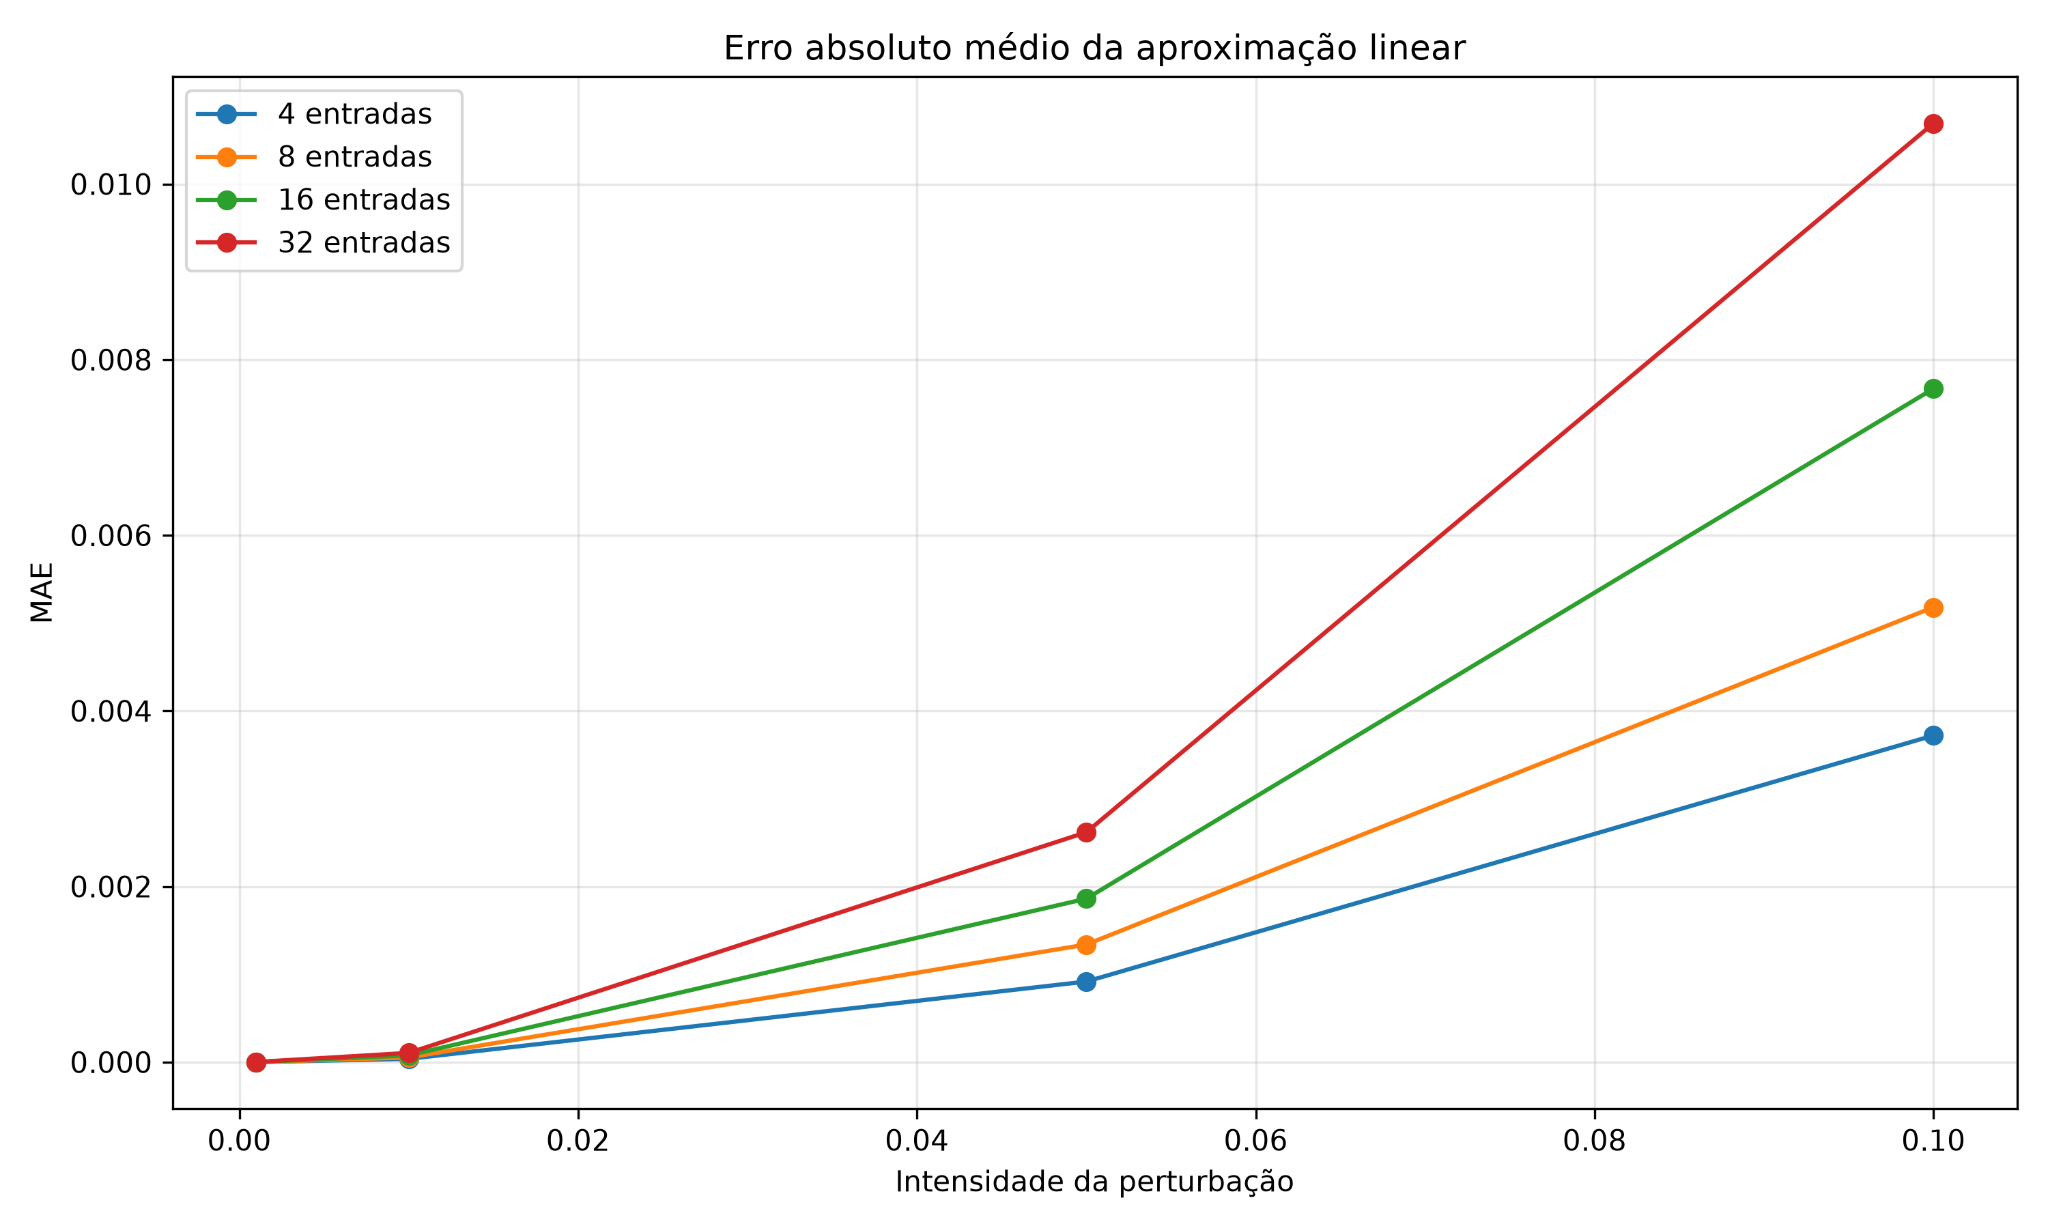
\includegraphics[width=0.94\textwidth]{grafico_erro_absoluto.png}
\caption{Erro absoluto médio da aproximação linear por intensidade de perturbação.}
\label{fig:mae}
\fonte{Elaboração própria a partir de \texttt{experimento\_resumo.csv}.}
\end{figure}

\begin{figure}[H]
\centering
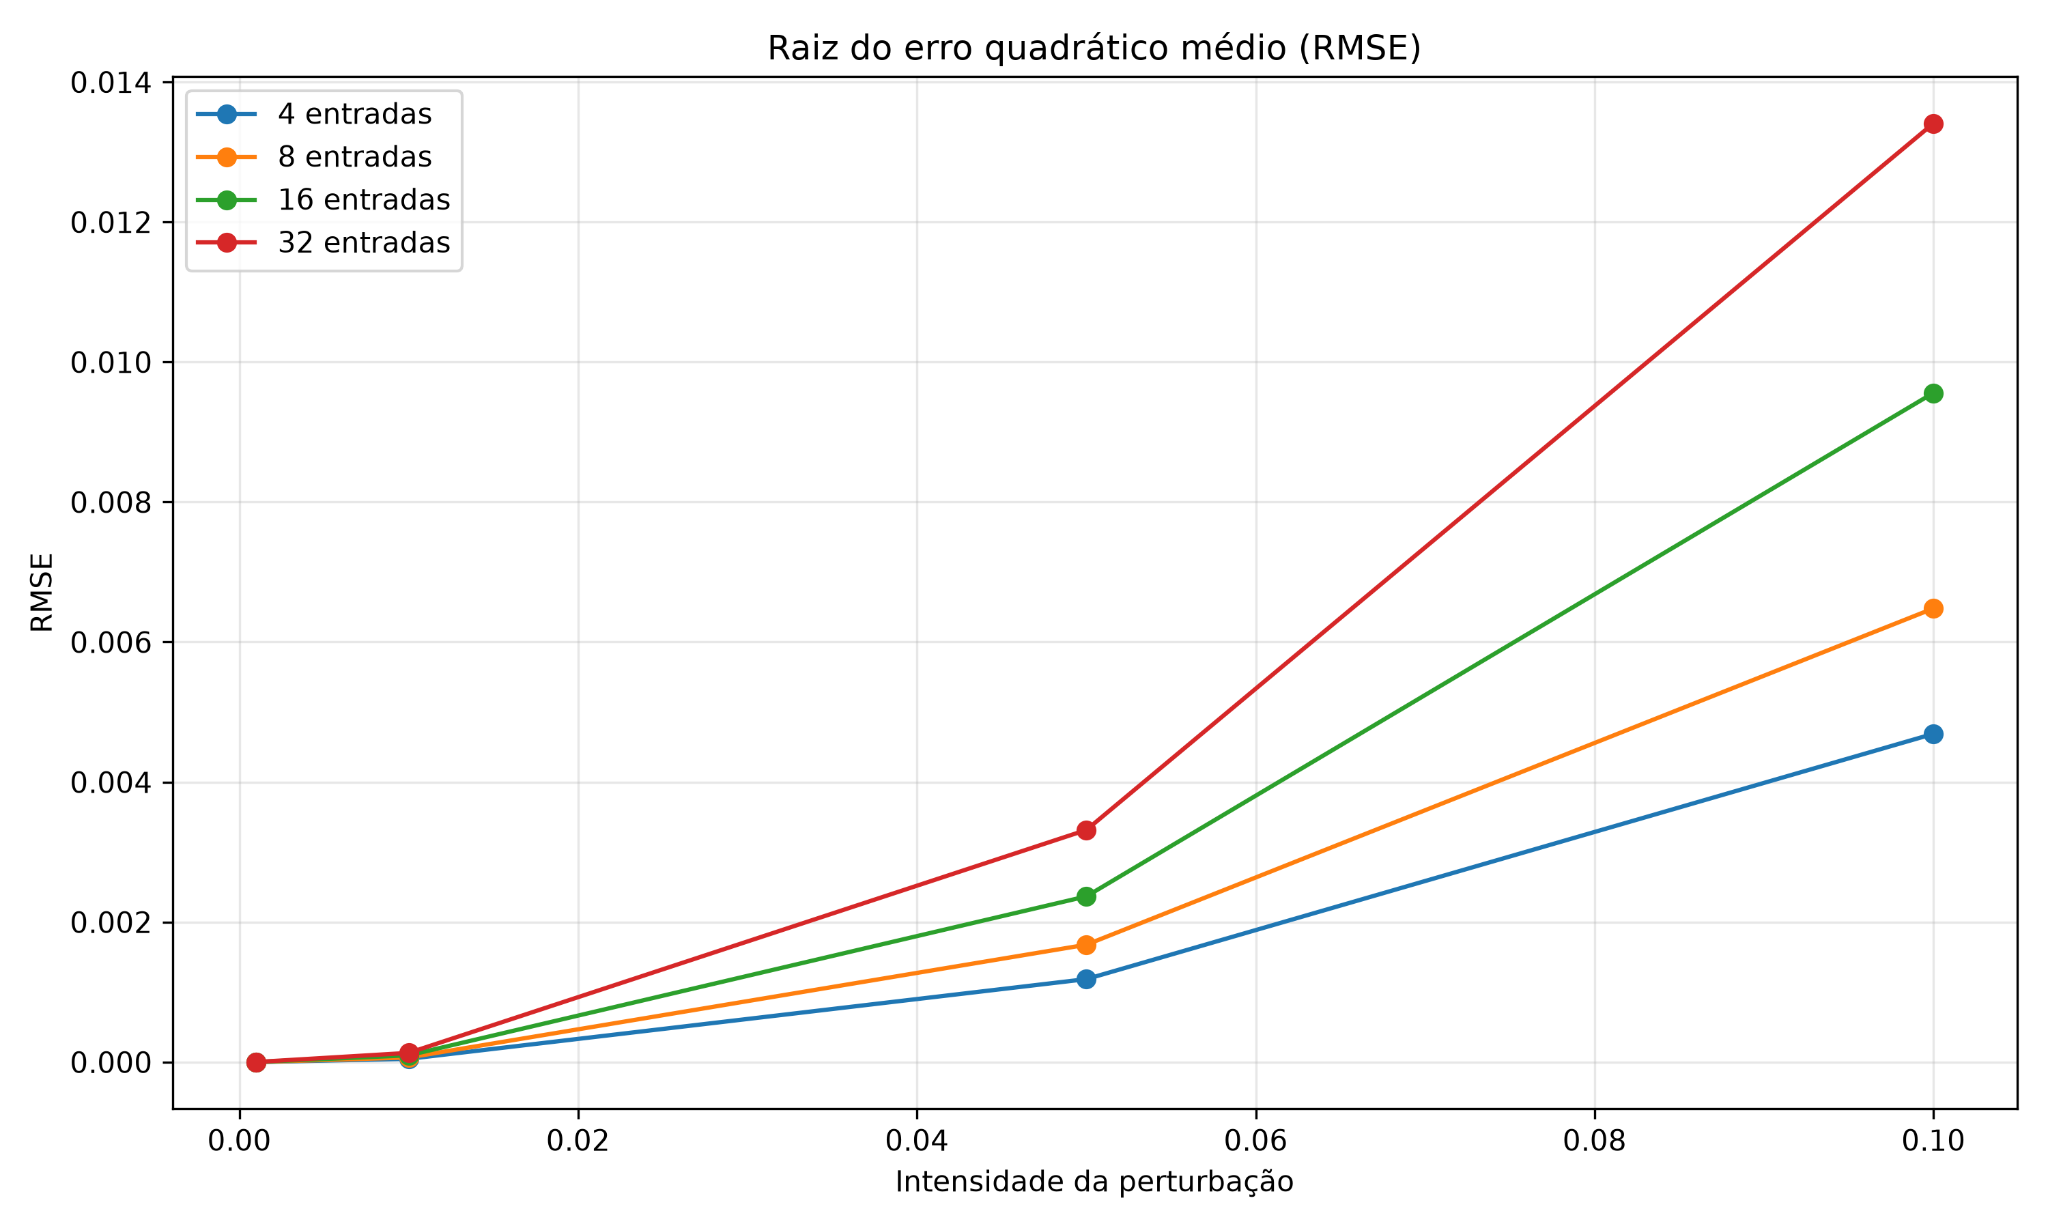
\includegraphics[width=0.94\textwidth]{grafico_rmse.png}
\caption{Raiz do erro quadrático médio do resíduo por intensidade de perturbação.}
\label{fig:rmse}
\fonte{Elaboração própria a partir de \texttt{experimento\_resumo.csv}.}
\end{figure}

A Figura~\ref{fig:mae} mostra que o MAE aumenta à medida que a intensidade cresce, e que os grafos com mais entradas apresentam resíduo absoluto médio maior. A Figura~\ref{fig:rmse} apresenta tendência correspondente para o RMSE, que penaliza mais fortemente resíduos de maior magnitude.

\begin{figure}[H]
\centering
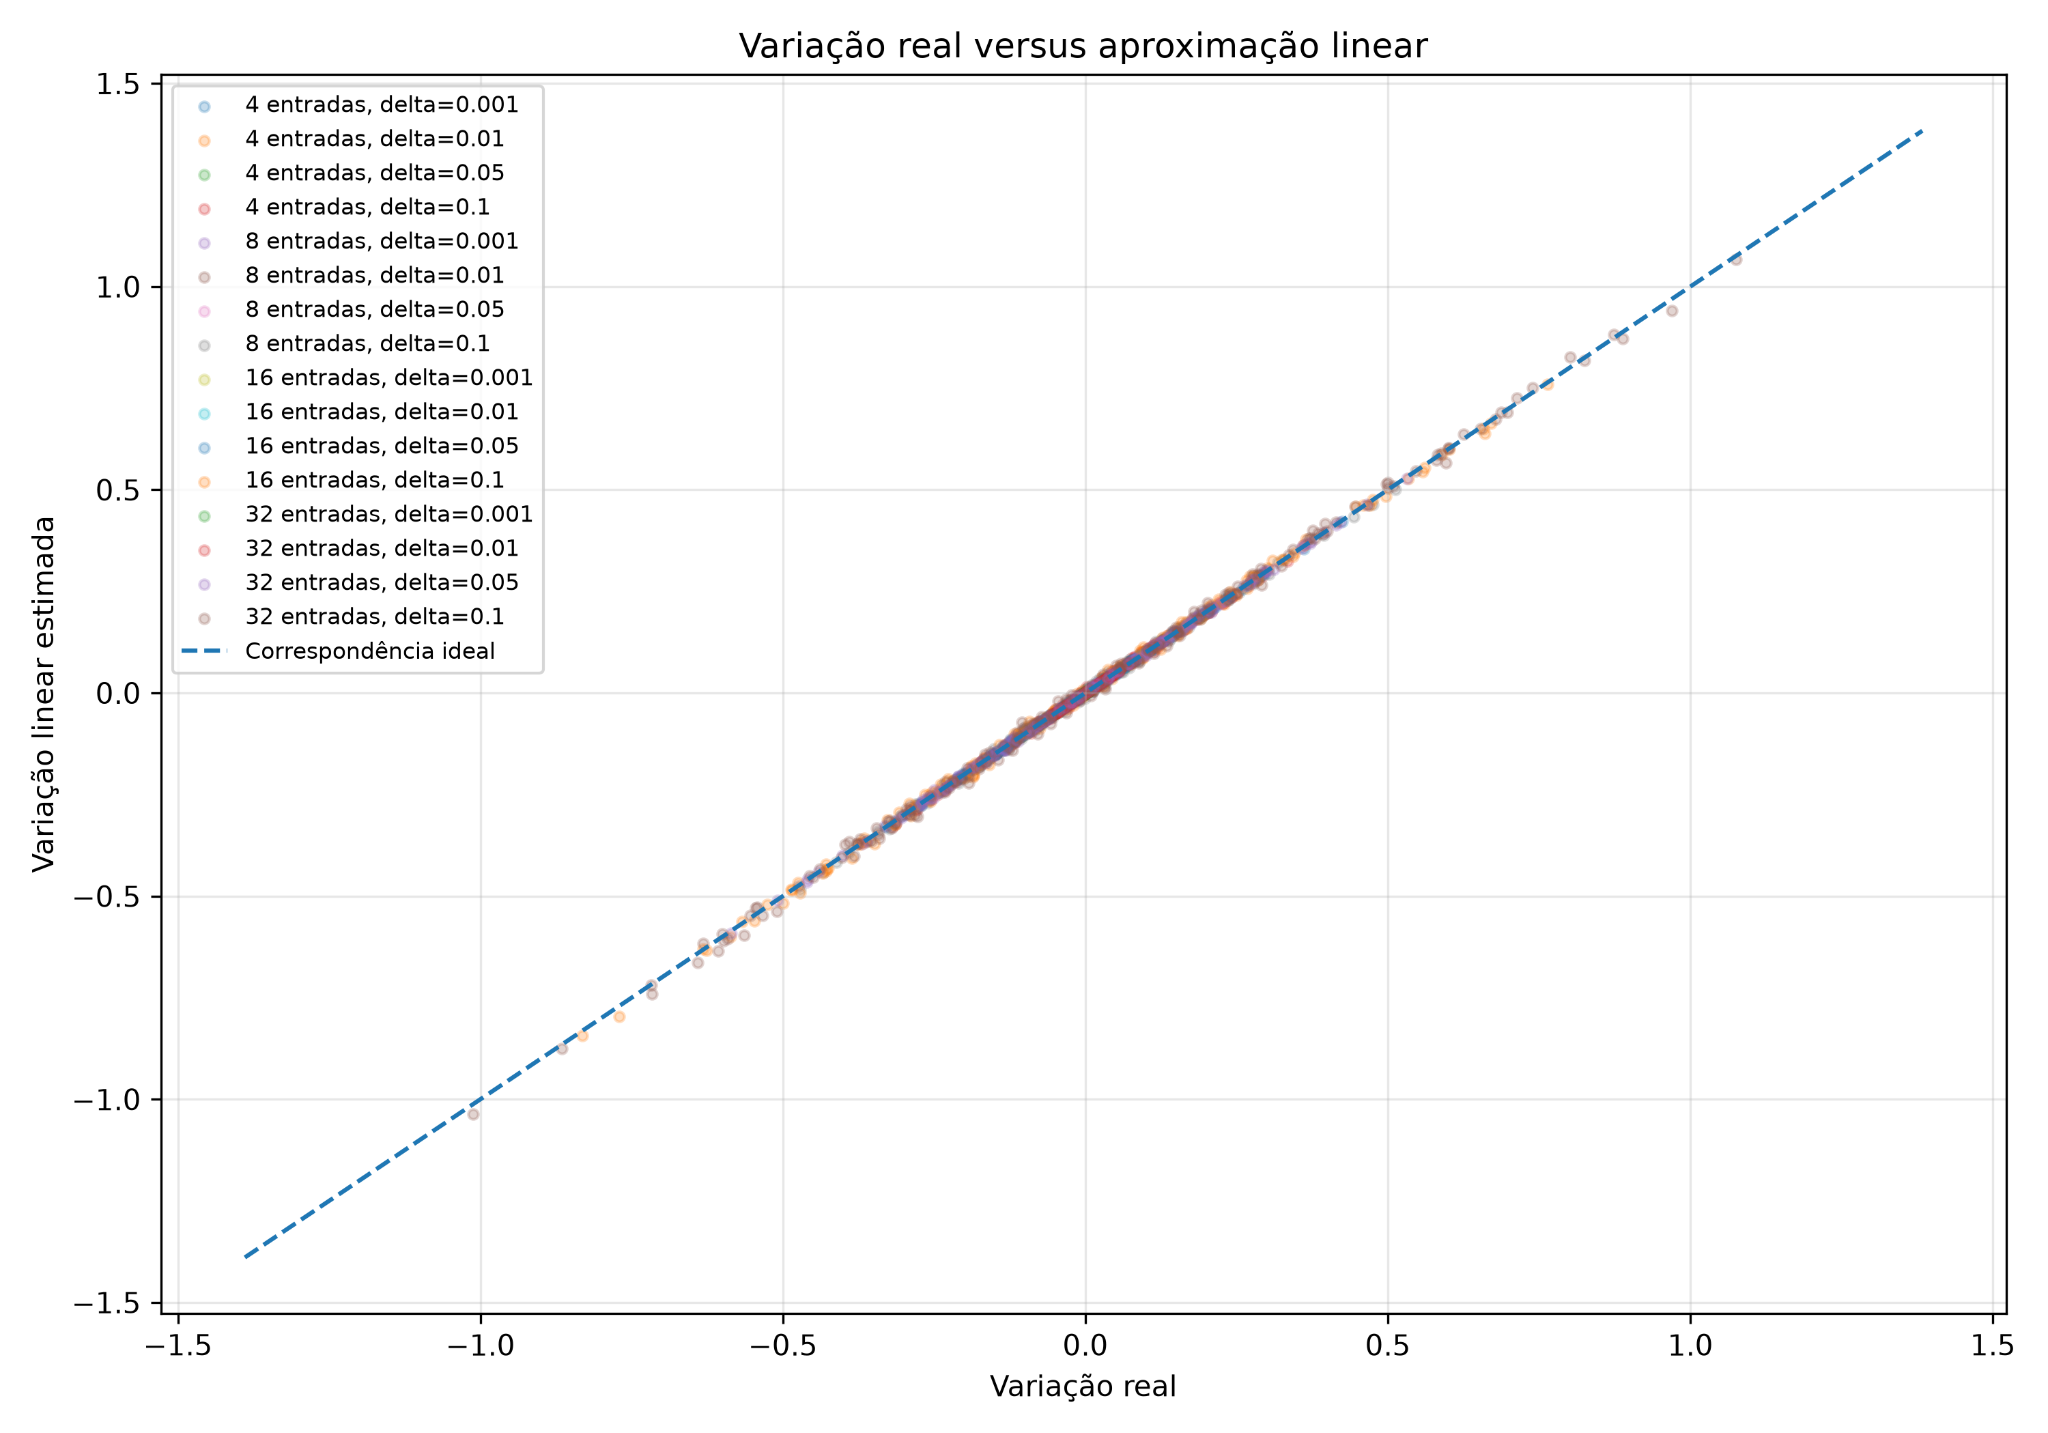
\includegraphics[width=0.94\textwidth]{grafico_real_vs_linear.png}
\caption{Variação real versus variação estimada pela aproximação linear.}
\label{fig:dispersao}
\fonte{Elaboração própria a partir de \texttt{experimento\_amostras.csv}.}
\end{figure}

Os pontos da Figura~\ref{fig:dispersao} ficam próximos da reta de correspondência ideal. Essa proximidade deve ser lida junto com as métricas de resíduo: a correlação elevada indica associação linear forte entre as variações, mas não significa igualdade ponto a ponto nem erro nulo.

\section{Dedução e confronto com a previsão teórica}
Para cada par, a função é $g_k(x_{2k},x_{2k+1})=x_{2k}x_{2k+1}$. Com perturbações aditivas,
\begin{align}
&(x_{2k}+\delta_{2k})(x_{2k+1}+\delta_{2k+1})-x_{2k}x_{2k+1}\\
&\quad=x_{2k}\delta_{2k+1}+x_{2k+1}\delta_{2k}+\delta_{2k}\delta_{2k+1}.
\end{align}
A aproximação de primeira ordem contém os dois termos lineares. Para $m=n/2$ produtos, o resíduo exato é
\begin{equation}
R=\sum_{k=0}^{m-1}\delta_{2k}\delta_{2k+1}.
\label{eq:residuo-par}
\end{equation}

Se as perturbações são independentes e uniformes em $[-d_a,d_a]$, então a esperança de cada perturbação é zero, e sua variância é $d_a^2/3$. Cada produto em \eqref{eq:residuo-par} possui esperança zero e segundo momento $d_a^4/9$. Como os pares são independentes,
\begin{equation}
E[R]=0,\qquad E[R^2]=\frac{m d_a^4}{9}.
\end{equation}
Logo, a previsão teórica para o RMSE do resíduo é
\begin{equation}
\mathrm{RMSE}_{\text{teórico}}=\sqrt{E[R^2]}=\frac{d_a^2\sqrt{m}}{3}=\frac{d_a^2\sqrt{n/2}}{3}.
\label{eq:rmse-teorico}
\end{equation}

A Tabela~\ref{tab:theory} compara a previsão com os valores empíricos. O desvio relativo observado variou de aproximadamente $-2{,}80\%$ a $+4{,}28\%$ nas 16 configurações. A diferença é compatível com a variabilidade amostral de uma simulação com 1.000 repetições por configuração.
\begin{table}[H]
\centering
\small
\caption{Desvio relativo máximo e mínimo entre RMSE empírico e teórico.}
\label{tab:theory}
\begin{tabular}{l r r r}
\toprule
Configuração & RMSE empírico & RMSE teórico & Desvio relativo\\
\midrule
n=8, $d_a=0{,}10$ & $6{,}480\e{-3}$ & $6{,}667\e{-3}$ & $-2{,}804\%$\\
n=16, $d_a=0{,}001$ & $9{,}832\e{-7}$ & $9{,}428\e{-7}$ & $+4{,}282\%$\\
\bottomrule
\end{tabular}
\fonte{Cálculos a partir de \texttt{experimento\_resumo.csv} e da Equação~\ref{eq:rmse-teorico}.}
\end{table}

\begin{figure}[H]
\centering
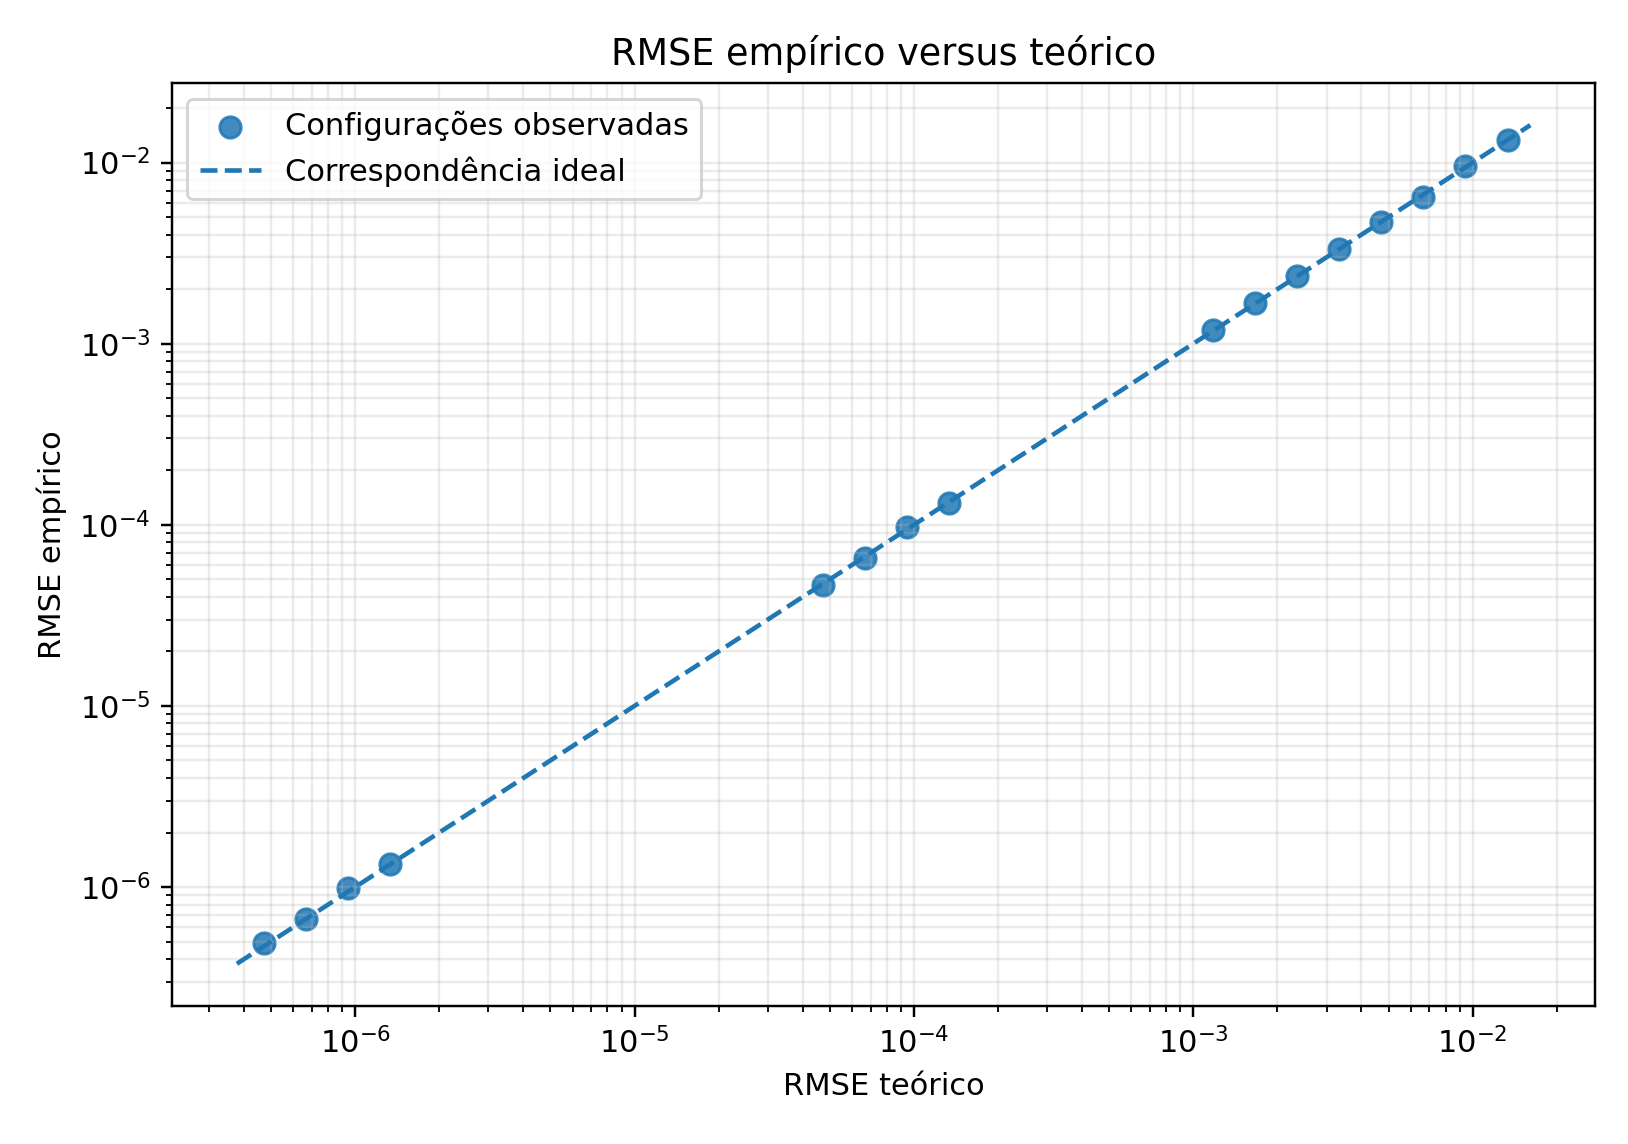
\includegraphics[width=0.90\textwidth]{rmse_empirico_teorico.png}
\caption{Comparação entre RMSE empírico e RMSE teórico.}
\label{fig:teoria}
\fonte{Elaboração própria a partir de \texttt{experimento\_resumo.csv}.}
\end{figure}

\section{Correlação e normalização dos erros}
A correlação de Pearson entre a variação real e a estimativa linear variou de 0,9993974347 a 0,9999999428. O menor valor ocorreu para 16 entradas e $d_a=0{,}10$; o maior, para 32 entradas e $d_a=0{,}001$. O erro relativo médio variou de aproximadamente 0,0335\% a 3,52\%, enquanto o maior NRMSE normalizado pela média do módulo da saída nominal foi de aproximadamente 0,1763\%.

A correlação elevada sustenta a proximidade do comportamento conjunto nos cenários avaliados, mas não substitui MAE ou RMSE. Uma transformação com escala ou viés sistemático também pode apresentar correlação alta; por isso, as métricas são interpretadas em conjunto.

\section{Verificação aritmética e reprodutibilidade dos resultados}
Foi realizada conferência das colunas dos 16.000 registros do CSV de amostras. Em cada linha, \texttt{residuo} coincide com \texttt{variacao\_real - variacao\_linear}; \texttt{erro\_absoluto} coincide com $|R|$; e \texttt{erro\_normalizado} coincide com $|R|/|o_{nominal}|$. A diferença máxima entre o resíduo armazenado e o recalculado foi nula na comparação numérica realizada; a diferença máxima na coluna do erro quadrático ficou na ordem de $2{,}71\times10^{-20}$, compatível com arredondamento de ponto flutuante.

As métricas MAE, MSE, RMSE, viés, NRMSE, erro relativo médio, mediana, percentil 95 e correlação foram recalculadas a partir das amostras. Os valores coincidiram com os 16 resumos, com diferença de correlação na ordem de $2{,}22\times10^{-16}$. A reexecução do script de precisão produziu o mesmo arquivo de resumo; no arquivo de amostras houve diferenças pontuais de representação em último dígito de ponto flutuante, sem alterar as métricas agregadas.

Essa conferência atesta a consistência aritmética interna dos arquivos, mas não substitui testes independentes do algoritmo. A validação do motor é sustentada também pelos casos analíticos e pelos 21 métodos de teste automatizado.

\section{Resultados do experimento abrangente}
Os arquivos de resultados do experimento contêm 384.000 linhas de amostras, 384 linhas de resumo e 384 intervalos de confiança para o MAE. Cada combinação dos fatores experimentais possui exatamente 1.000 amostras: quatro operações, duas estruturas, quatro tamanhos, quatro intensidades e três tipos de perturbação. O campo \texttt{amostras\_validas} registra 1.000 em todas as combinações, e \texttt{amostras\_invalidas} registra zero. Portanto, as 384.000 amostras foram consideradas válidas pelo próprio experimento.

A auditoria final também padronizou o sinal do resíduo assinado. Em cada linha, \texttt{erro\_assinado} corresponde a $\Delta o_{\mathrm{real}}-\Delta o_{\mathrm{lin}}$; em cada configuração, \texttt{Vies} corresponde à média desses resíduos. A correção foi feita por inversão de sinal nas duas colunas, preservando as variações real e linear e as 384.000 simulações já realizadas. Como MAE, MSE, RMSE, NRMSE, MAPE, P95, correlação e intervalos dependem de módulos, quadrados ou erros absolutos, seus valores permaneceram inalterados. O script \texttt{validar\_residuos\_abrangente.py} verifica essa identidade nas amostras e nos 384 resumos.

A Tabela~\ref{tab:abrangente-operacoes} resume, para cada operação, a mediana do RMSE e da NRMSE, a mediana do MAPE e a menor correlação observada nas 96 configurações daquela operação. O RMSE é uma medida absoluta e depende da escala dos resultados; por isso, seus valores não devem ser comparados isoladamente entre operações com magnitudes nominais muito diferentes. A NRMSE utilizada pelo script divide o RMSE pela amplitude das variações reais, e não pelo valor nominal da saída.

\begin{table}[H]
\centering
\small
\caption{Síntese das métricas por operação no experimento abrangente.}
\label{tab:abrangente-operacoes}
\begingroup
\scriptsize
\setlength{\tabcolsep}{3pt}
\begin{tabular}{lrrrrr}
\toprule
Operação & RMSE med. & RMSE máx. & NRMSE med. & MAPE med. (\%) & Corr. mín.\\
\midrule
ADD & $3{,}00\times10^{-15}$ & $1{,}84\times10^{-14}$ & $1{,}17\times10^{-14}$ & $2{,}64\times10^{-12}$ & 1,00000\\
SUB & $5{,}91\times10^{-16}$ & $1{,}26\times10^{-14}$ & $5{,}09\times10^{-15}$ & $2{,}85\times10^{-12}$ & 1,00000\\
MUL & $6{,}17\times10^{1}$ & $6{,}13\times10^{12}$ & 0,04549 & 11,13 & 0,95817\\
DIV & $2{,}18\times10^{-5}$ & $1{,}08\times10^{-1}$ & 0,01203 & 5,59 & 0,95861\\
\bottomrule
\end{tabular}
\endgroup
\fonte{Cálculos a partir de \texttt{abrangente\_resumo.csv}; cada mediana considera as 96 combinações correspondentes à operação.}
\end{table}

Para ADD e SUB, o resíduo permaneceu na ordem de $10^{-15}$, compatível com arredondamento de ponto flutuante. Esse resultado é esperado: em aritmética real, cada grafo homogêneo formado apenas por adições ou apenas por subtrações representa uma função afim das entradas, cuja variação é descrita exatamente pela primeira ordem. Portanto, esses dois conjuntos não demonstram por si só a precisão do método em funções não lineares; eles verificam a consistência da implementação e o nível residual decorrente da aritmética de ponto flutuante. Já MUL e DIV são não lineares; para essas operações, os termos de ordem superior não desaparecem e o erro depende da intensidade, da quantidade de entradas, da estrutura e do padrão de sinais.

O maior RMSE de todo o experimento ocorreu em MUL, cadeia, 32 entradas, intensidade de 10\% e perturbação positiva: $6{,}1266\times10^{12}$. Nessa configuração, a saída nominal é aproximadamente $9{,}0829\times10^{11}$; a variação real observada ficou entre aproximadamente $6{,}4097\times10^{12}$ e $1{,}0344\times10^{13}$, enquanto a estimativa linear ficou entre $1{,}9609\times10^{12}$ e $2{,}3807\times10^{12}$. A aproximação subestimou sistematicamente a variação real nesse cenário, apesar da correlação de 0,99863. Esse exemplo mostra por que a correlação não deve ser interpretada sozinha como medida de precisão.

O menor valor de correlação ocorreu em MUL, ramificada, 32 entradas, intensidade de 10\% e perturbação combinada: 0,95817, com RMSE de aproximadamente $1{,}1524\times10^{11}$ e MAPE de 259,63\%. O maior MAPE, 283,14\%, ocorreu em DIV, cadeia, oito entradas, intensidade de 5\% e perturbação combinada. Esse percentual elevado deve ser interpretado com cautela porque o MAPE divide o erro pela magnitude da variação real; quando essa variação está próxima de zero, o quociente pode crescer mesmo quando o erro absoluto é pequeno.

A NRMSE ficou indefinida em sete configurações porque a amplitude das variações reais não ultrapassou $10^{-12}$. O MAPE ficou indefinido em cinco configurações porque nenhuma amostra da configuração satisfez o limite $|\Delta o_{\mathrm{real}}|>10^{-12}$. Essas ocorrências não são amostras inválidas: as 384.000 amostras foram aceitas, e apenas as métricas normalizadas ficaram sem denominador adequado. A NRMSE máxima foi 34,71, em MUL, cadeia, 32 entradas, 10\% e perturbação negativa; nesse caso, o RMSE foi cerca de 34,7 vezes a amplitude das variações reais, evidenciando baixa adequação da estimativa linear nessa normalização específica.

\begin{figure}[H]
\centering
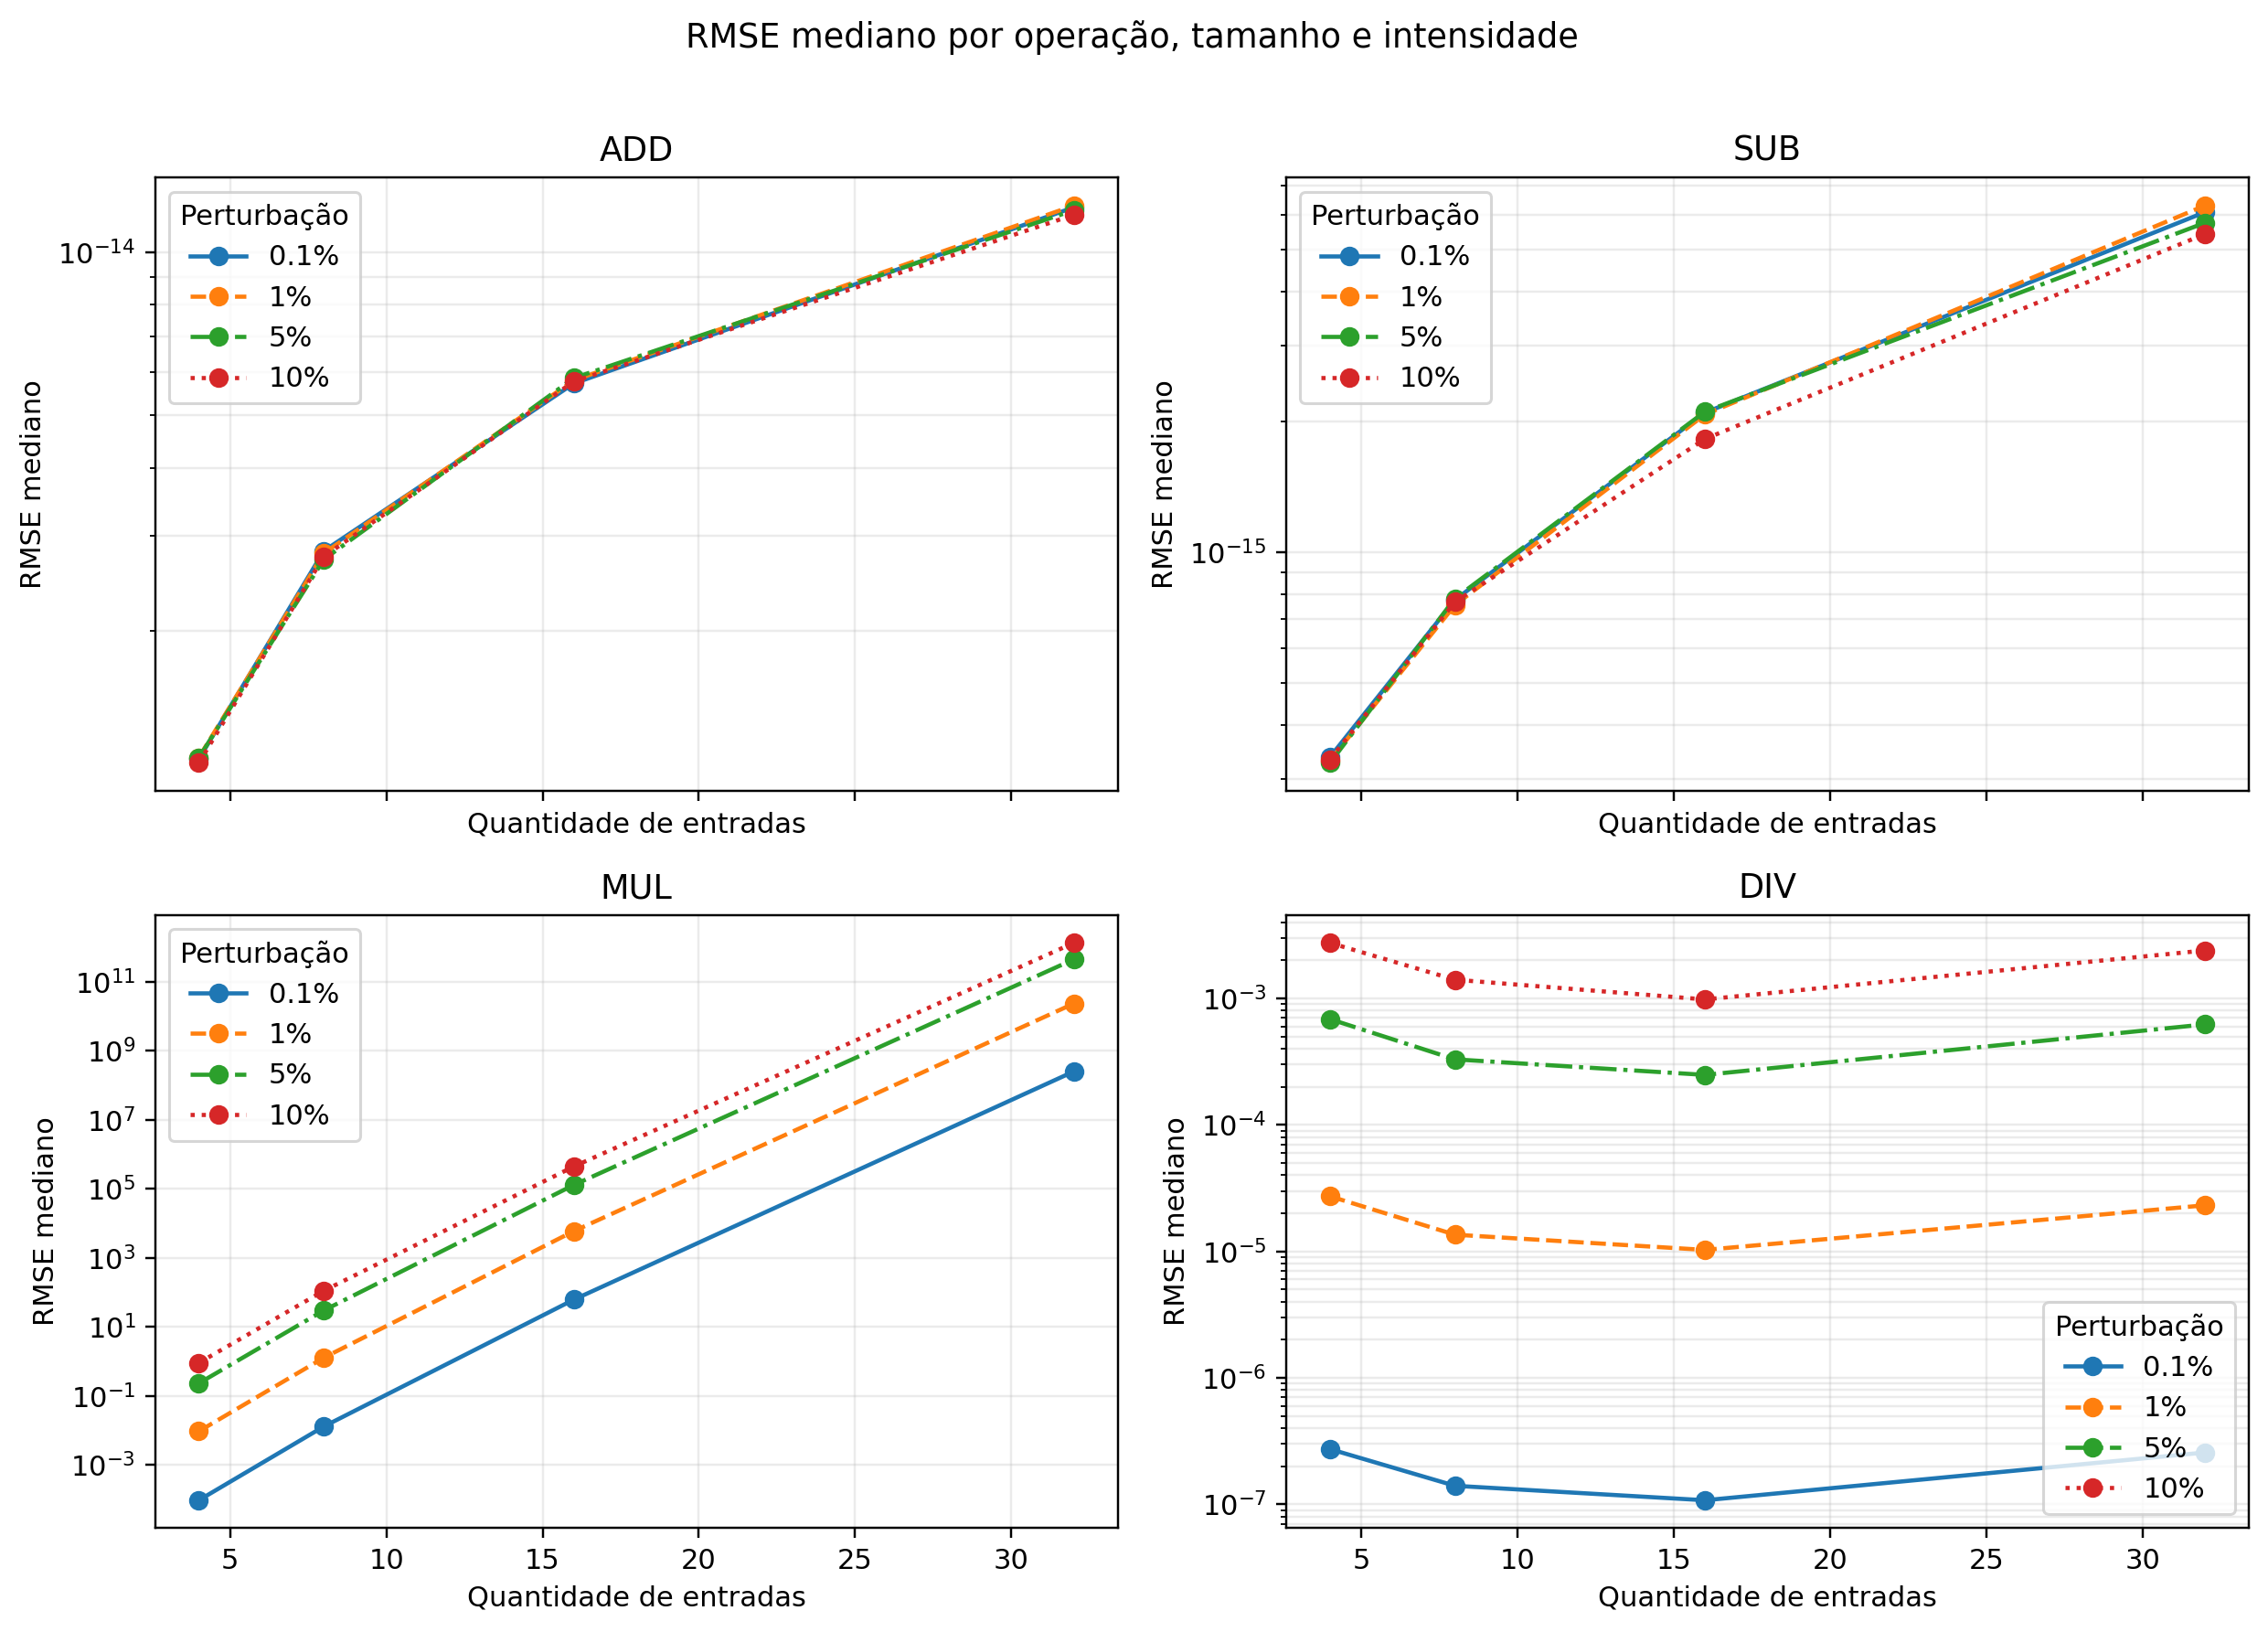
\includegraphics[width=0.96\textwidth]{abrangente_rmse_operacao_tamanho.png}
\caption{RMSE mediano por operação, tamanho do grafo e intensidade de perturbação. Eixo vertical em escala logarítmica.}
\label{fig:abrangente-rmse}
\fonte{Elaboração própria a partir de \texttt{abrangente\_resumo.csv}. Cada ponto representa a mediana de seis configurações (duas estruturas e três tipos de perturbação).}
\end{figure}

\begin{figure}[H]
\centering
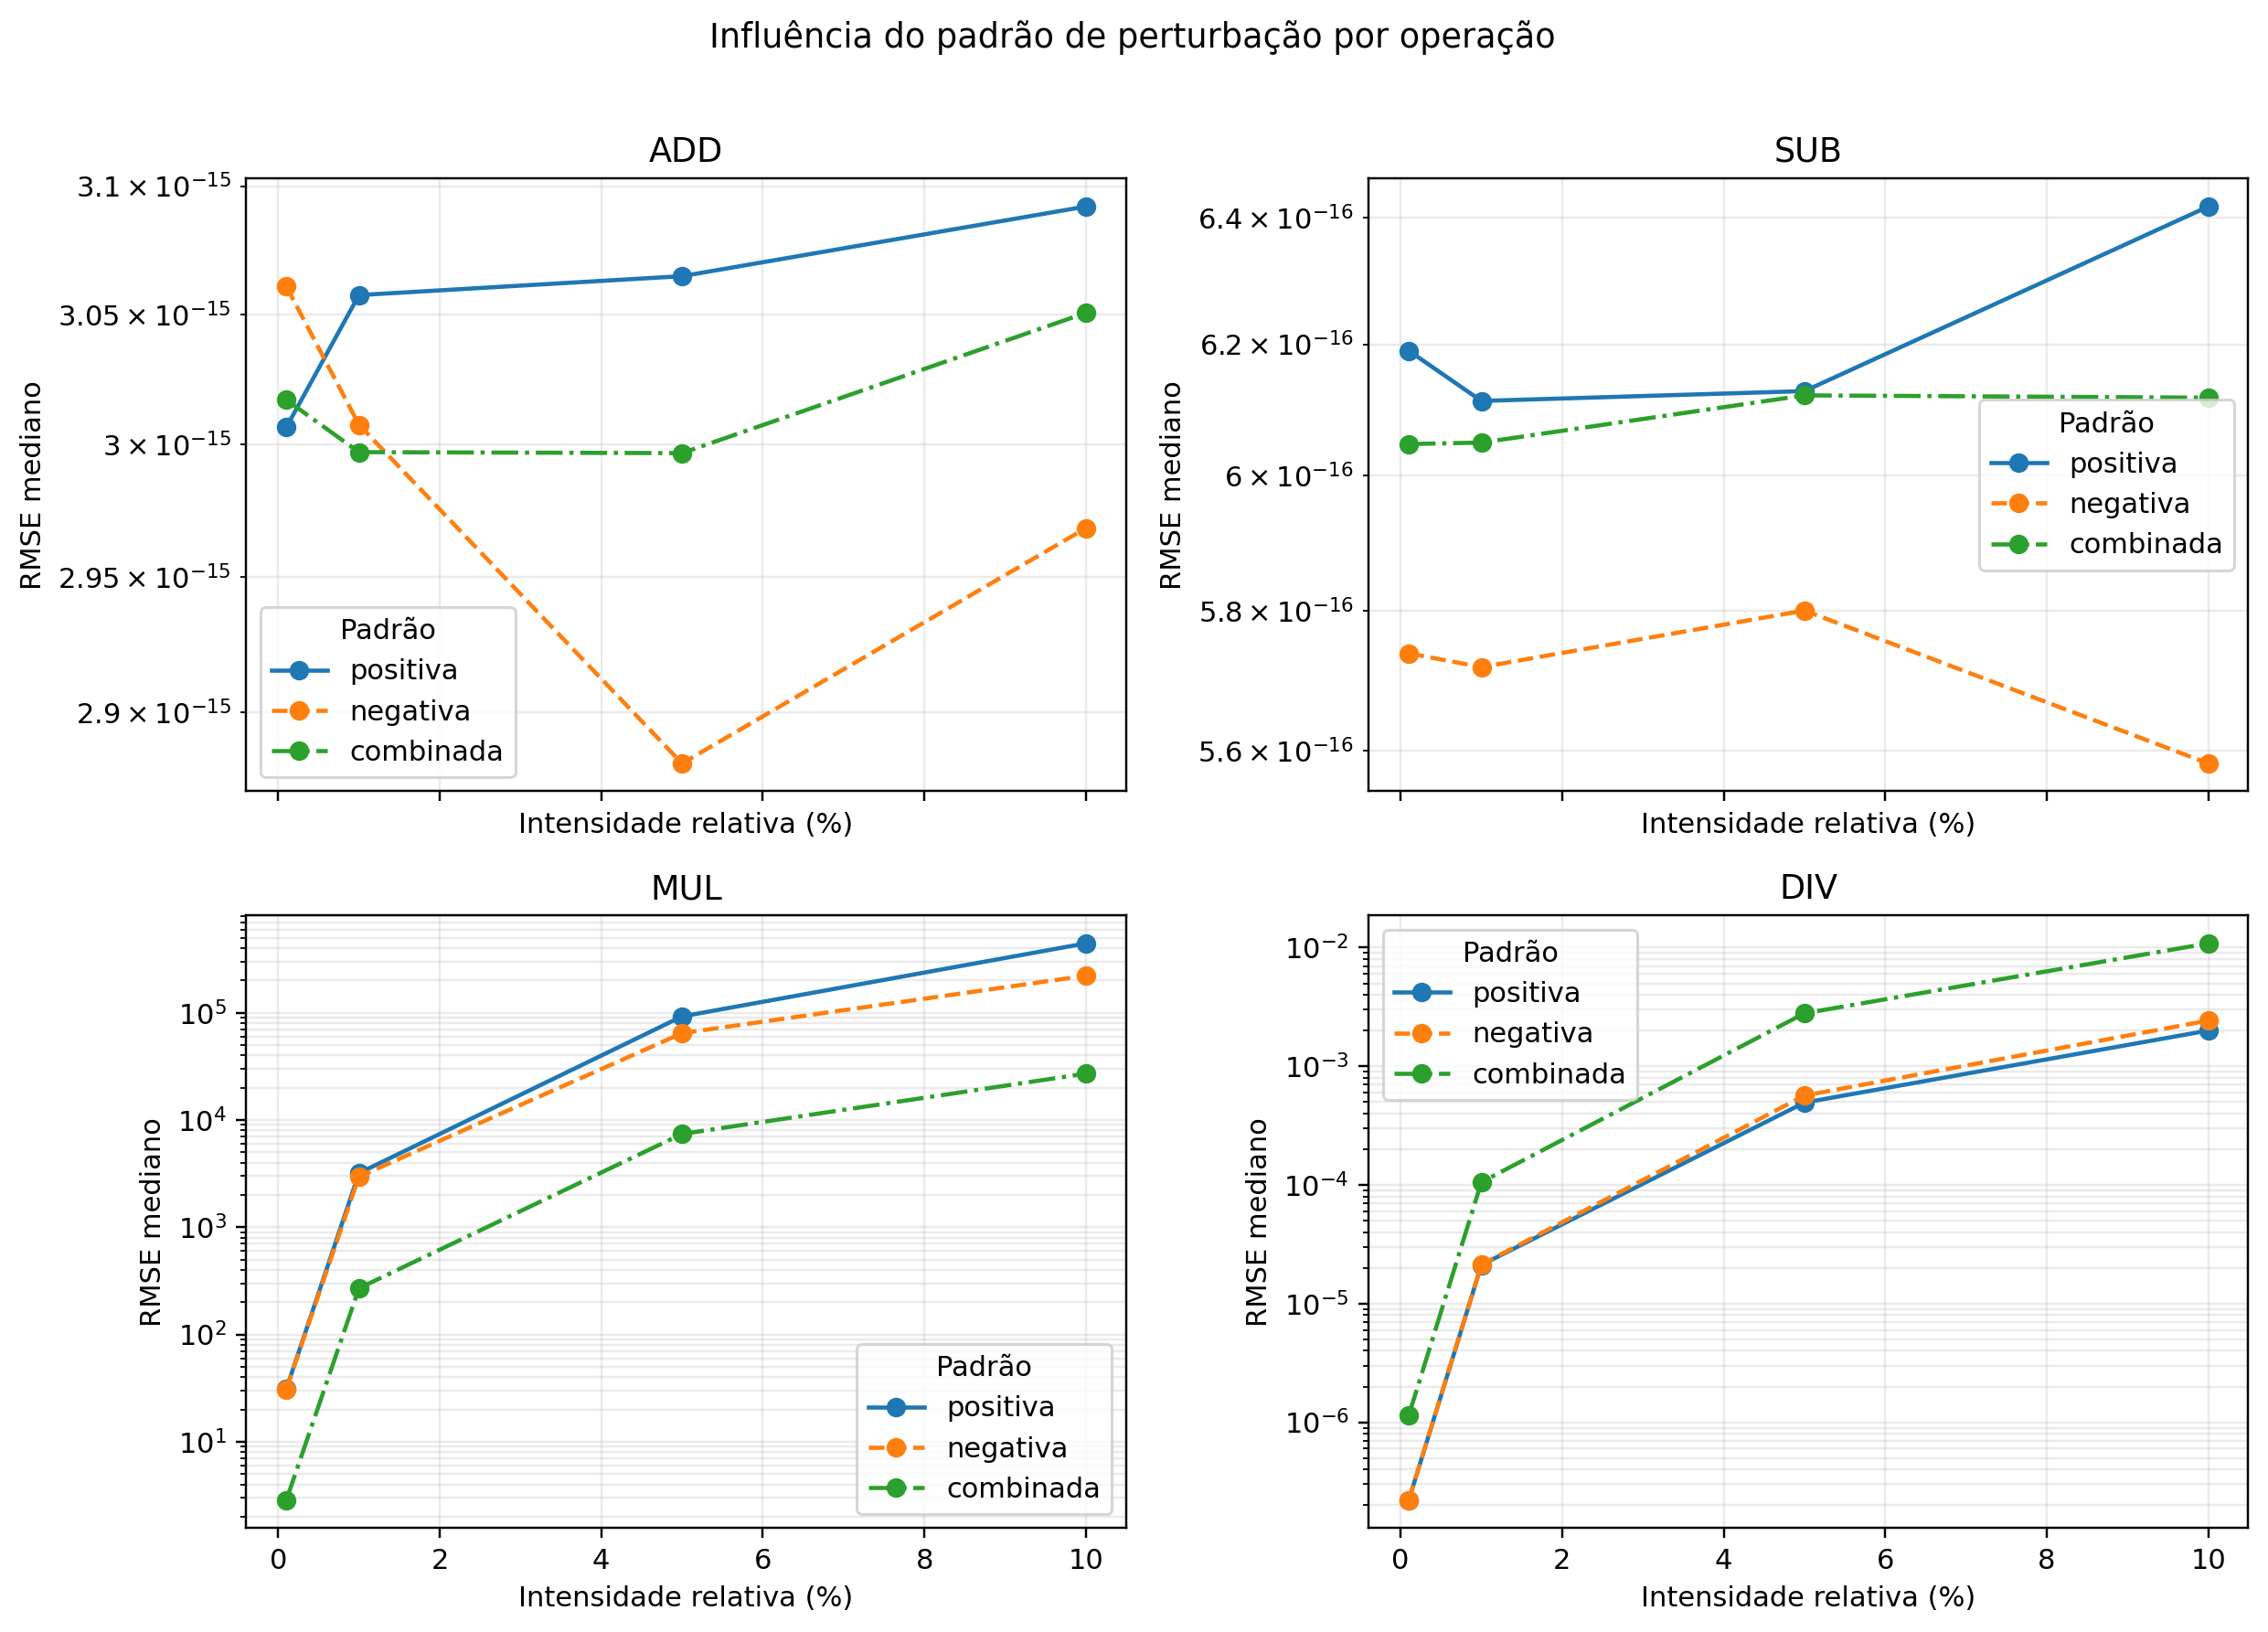
\includegraphics[width=0.96\textwidth]{abrangente_sentido_por_operacao.png}
\caption{Influência do sentido da perturbação no RMSE, apresentada separadamente para cada operação.}
\label{fig:abrangente-sentido}
\fonte{Elaboração própria a partir de \texttt{abrangente\_resumo.csv}. Cada ponto representa a mediana sobre os tamanhos e as duas estruturas, para uma operação, intensidade e tipo de perturbação.}
\end{figure}

A Figura~\ref{fig:abrangente-sentido} permite observar que o sentido da perturbação não produz um efeito uniforme entre operações. Em multiplicações com muitas entradas, perturbações de mesmo sinal podem acumular seus efeitos sobre o produto, enquanto sinais combinados podem produzir compensações parciais. Essa compensação não garante melhor aproximação em todos os cenários: para MUL com 32 entradas e 10\% de perturbação combinada, a correlação foi justamente a menor do experimento.

\begin{figure}[H]
\centering
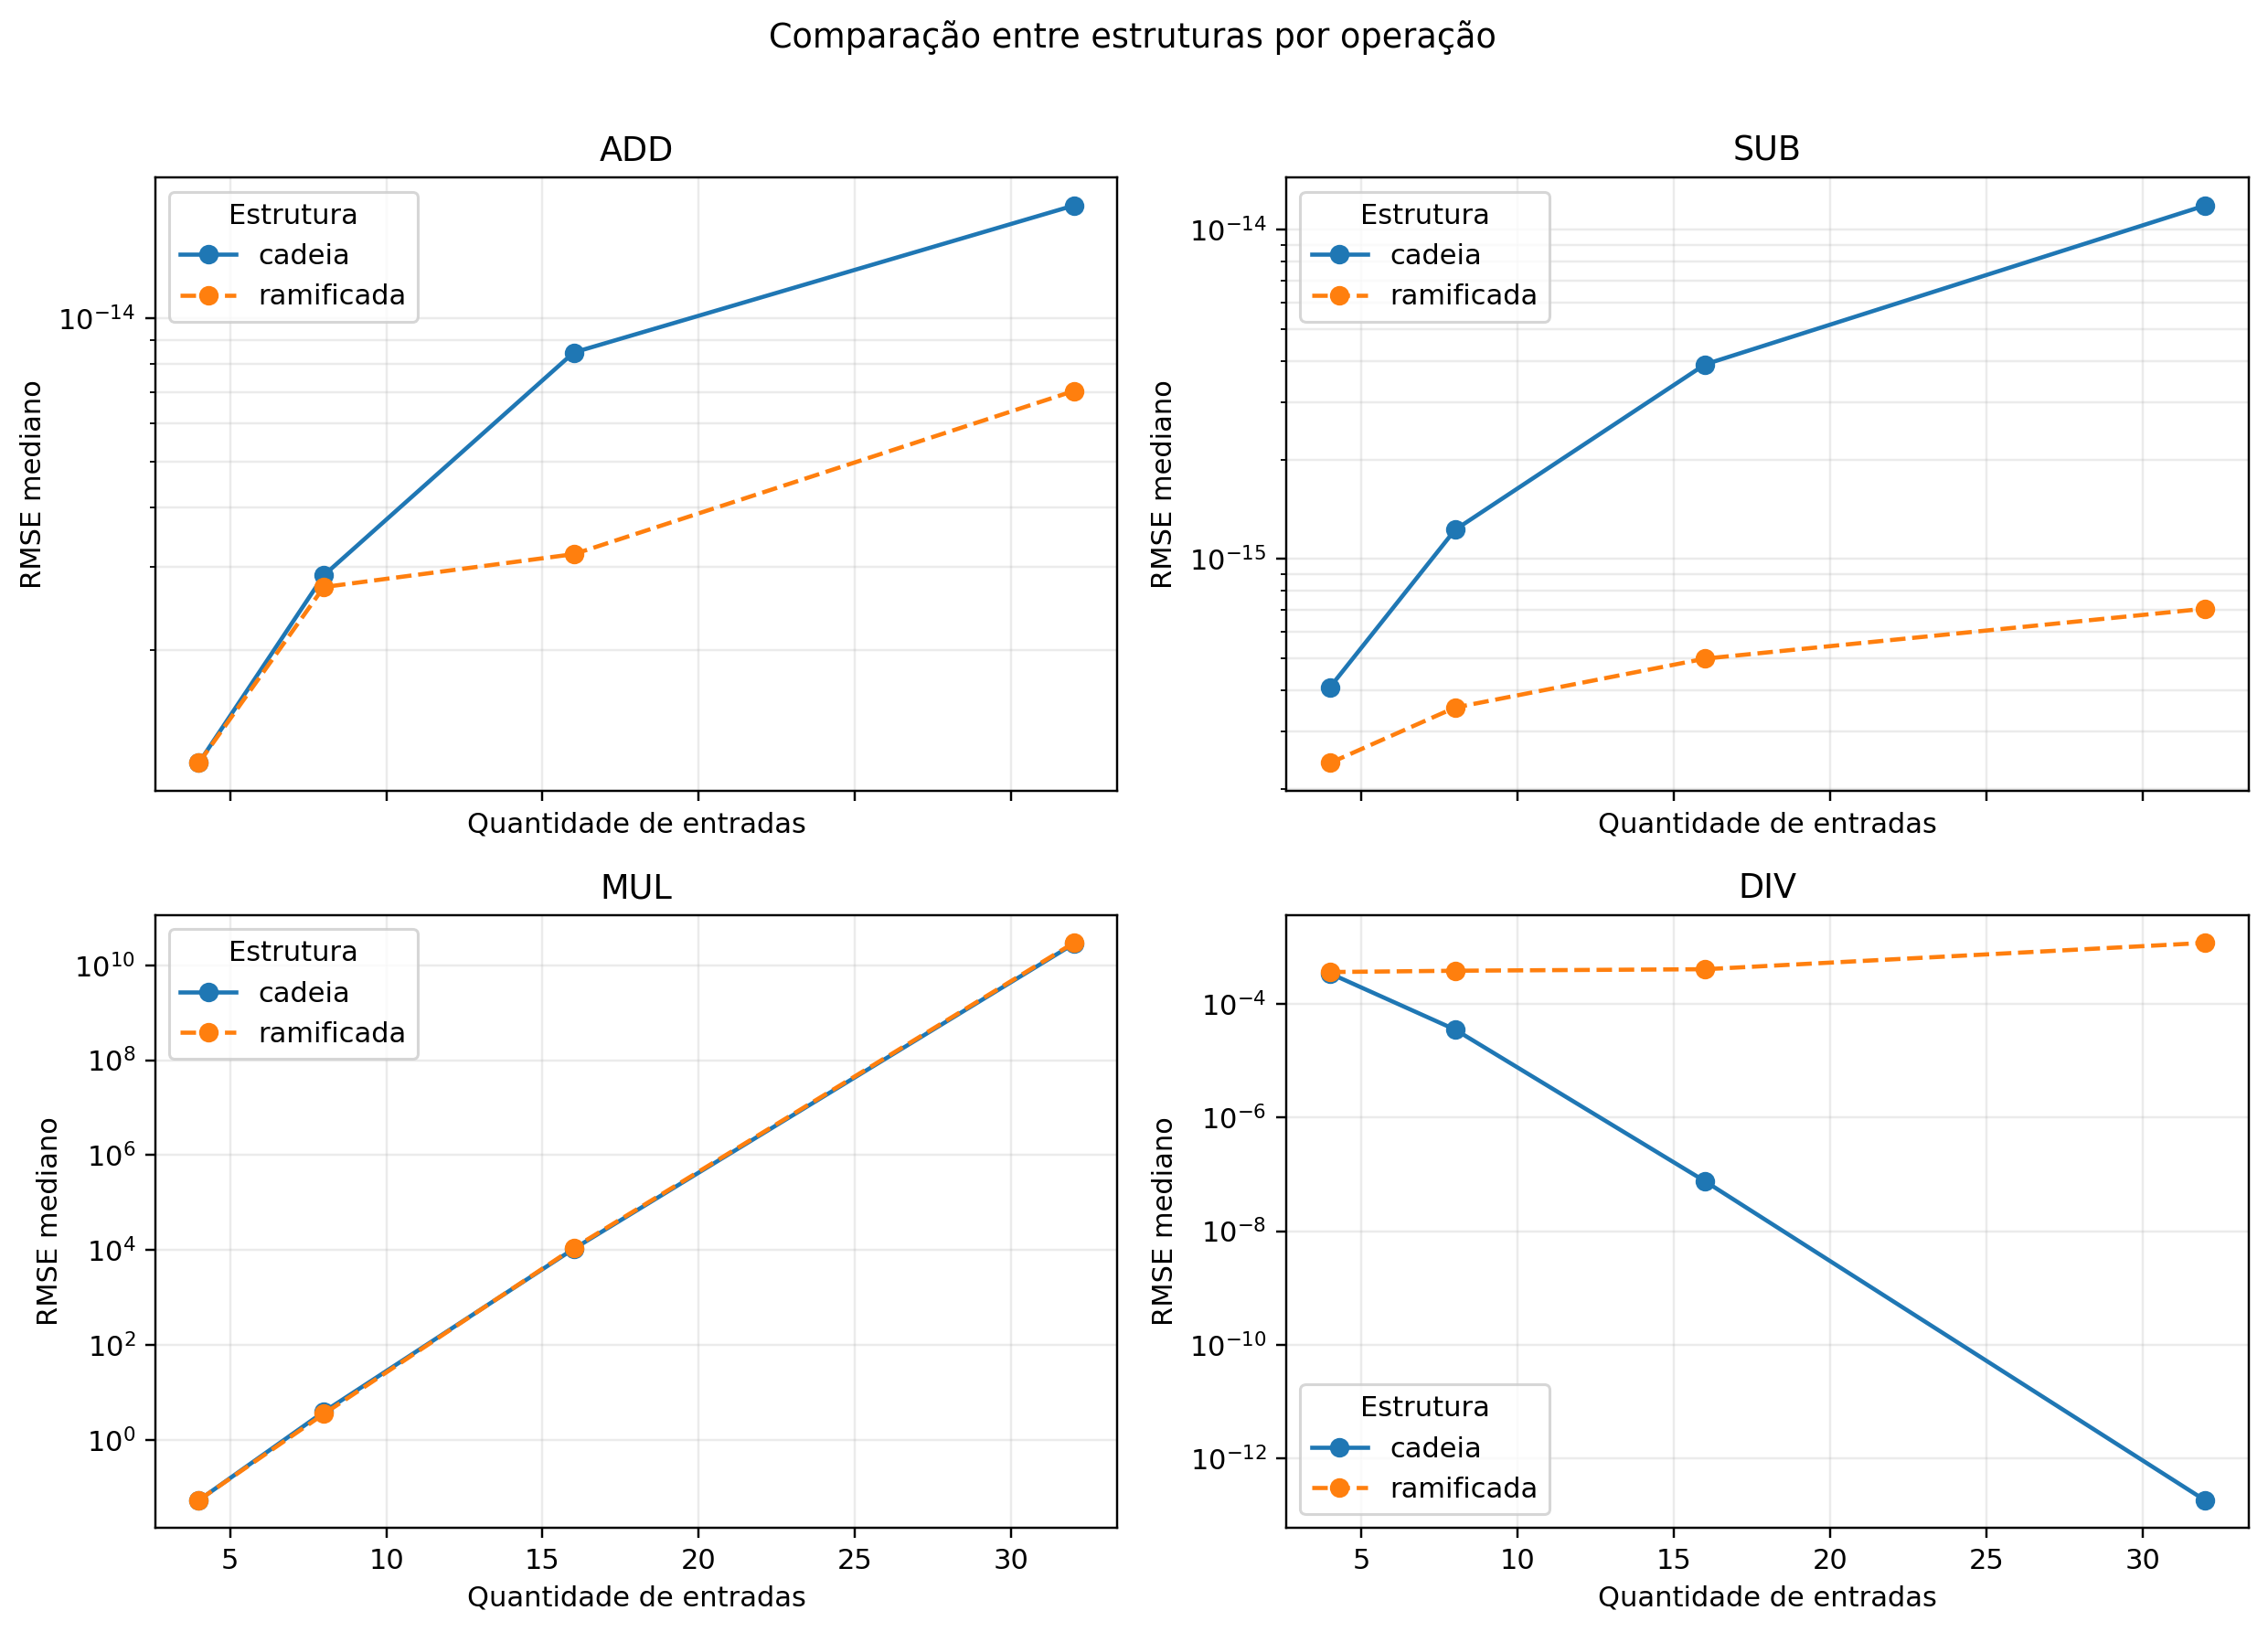
\includegraphics[width=0.96\textwidth]{abrangente_estrutura_por_operacao.png}
\caption{Comparação entre as estruturas em cadeia e ramificada, separada por operação.}
\label{fig:abrangente-estrutura}
\fonte{Elaboração própria a partir de \texttt{abrangente\_resumo.csv}. Cada ponto representa a mediana sobre as quatro intensidades e os três tipos de perturbação.}
\end{figure}

A comparação da Figura~\ref{fig:abrangente-estrutura} deve ser interpretada à luz da associação das operações. Para ADD e MUL, cadeia e árvore ramificada representam a mesma expressão matemática em aritmética exata, embora a ordem de avaliação possa produzir pequenas diferenças de ponto flutuante. Para SUB e DIV, as operações não são associativas; a cadeia à esquerda e a árvore balanceada representam expressões diferentes. Logo, os resultados com SUB e DIV comparam simultaneamente formato do grafo e parentização da expressão, não permitindo atribuir toda diferença exclusivamente à topologia.

No caso de DIV em cadeia, o RMSE absoluto mediano diminui de aproximadamente $3{,}39\times10^{-4}$ para quatro entradas a $1{,}85\times10^{-13}$ para 32 entradas. Essa queda não indica, por si só, melhora da aproximação. Como a cadeia aplica divisões sucessivas a entradas positivas iguais ou maiores que 2, a saída nominal diminui de cerca de $1{,}46\times10^{-1}$ para $4{,}40\times10^{-12}$ nos mesmos tamanhos. O resíduo absoluto acompanha essa redução de escala. A mediana da NRMSE, por sua vez, passa de aproximadamente 0,0142 para 0,1036 entre quatro e 16 entradas, antes de assumir 0,0642 em 32 entradas; portanto, a métrica normalizada não confirma uma melhora monotônica. A interpretação da Figura 8 deve considerar simultaneamente a escala da saída e as métricas normalizadas, além da diferença de parentização entre cadeia e árvore ramificada.

O gráfico de dispersão originalmente produzido pelo script usa as primeiras 5.000 linhas do arquivo na ordem de geração. Como a geração percorre primeiro as operações e as configurações, essa seleção não constitui uma amostra representativa de todas as 384 combinações. Para evitar essa limitação, foi construído um gráfico adicional com amostragem estratificada: oito observações selecionadas de cada combinação, totalizando 3.072 pontos, com um painel separado para cada operação.

\begin{figure}[H]
\centering
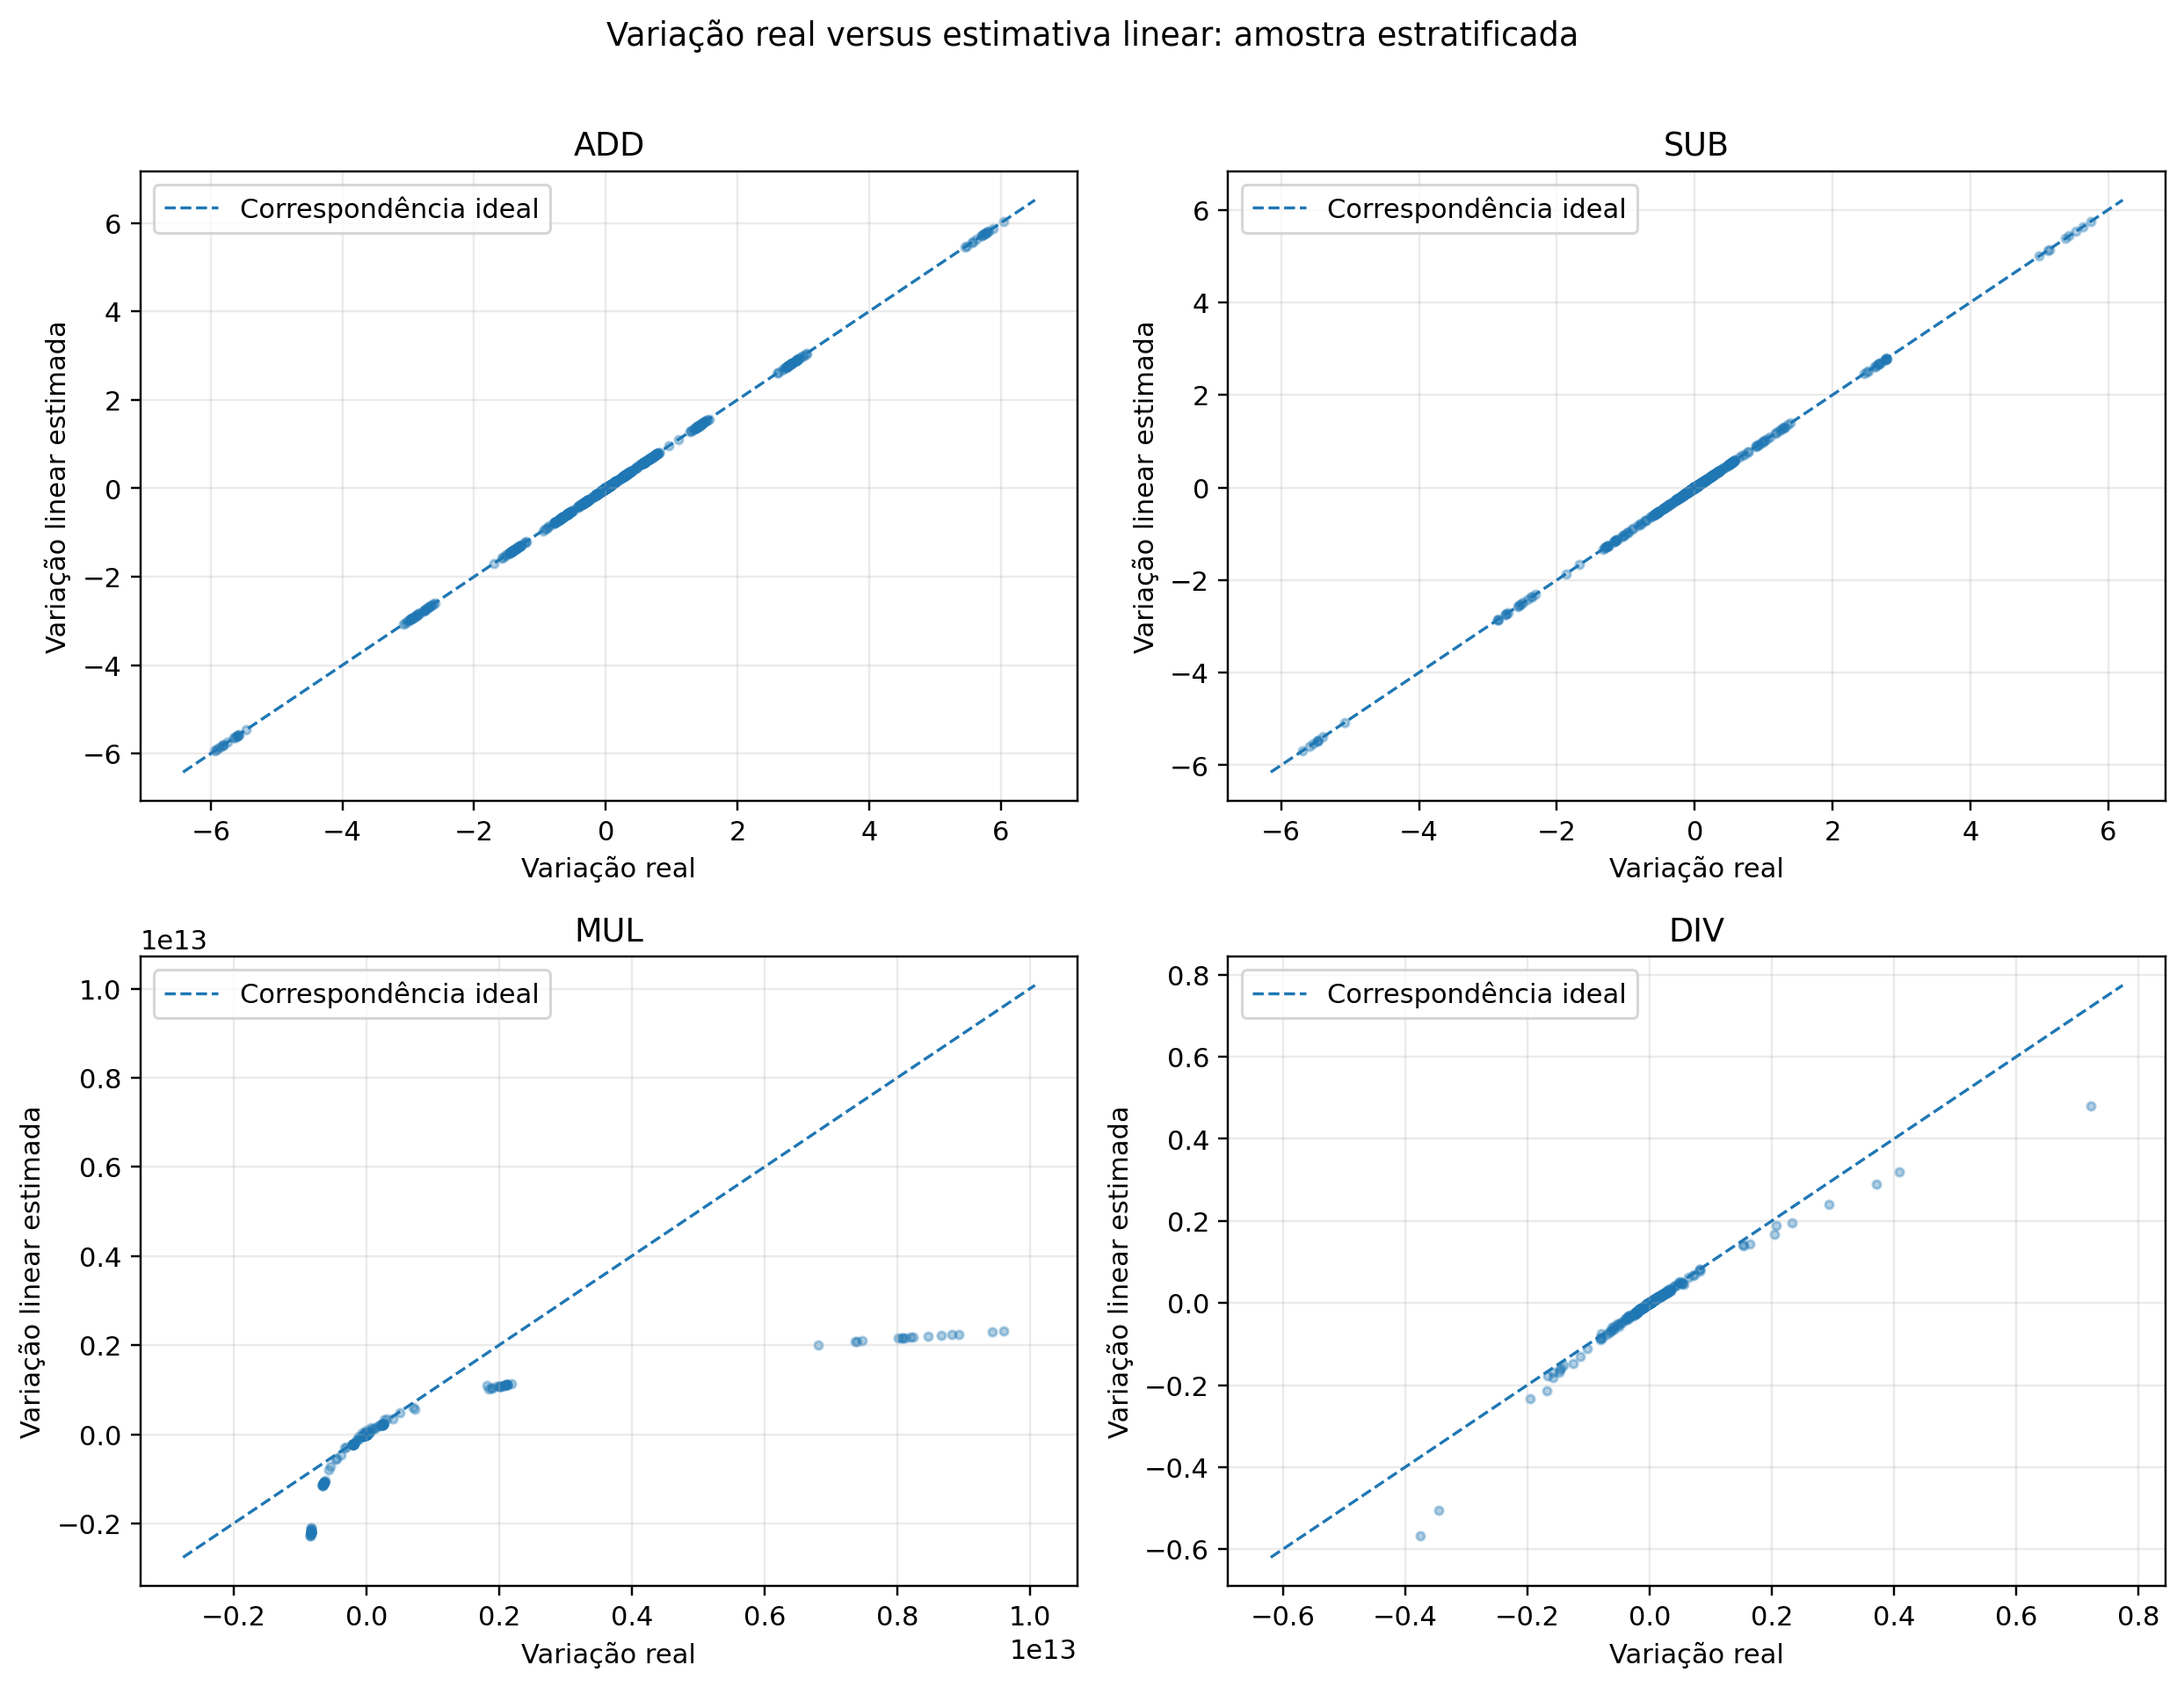
\includegraphics[width=0.96\textwidth]{abrangente_real_vs_linear_estratificado.png}
\caption{Variação real versus estimativa linear com amostragem estratificada por configuração e separação por operação.}
\label{fig:abrangente-dispersao}
\fonte{Elaboração própria a partir de \texttt{abrangente\_amostras.csv}; oito amostras foram selecionadas em cada uma das 384 configurações, com semente 20261110.}
\end{figure}

A Figura~\ref{fig:abrangente-dispersao} confirma visualmente a proximidade entre variação real e linear para ADD e SUB e evidencia desvios mais relevantes para MUL e DIV. Mesmo quando os pontos permanecem associados à reta ideal, os resíduos absolutos podem ser relevantes devido à escala dos resultados, como demonstrado no cenário de multiplicação com 32 entradas e perturbações positivas de 10\%.

\section{Discussão do experimento abrangente}
Os resultados permitem distinguir o comportamento das operações afins e não lineares. Para ADD e SUB, a primeira ordem reproduz a variação matemática exata, e os resíduos remanescentes são compatíveis com a aritmética de ponto flutuante da implementação. Para MUL e DIV, os termos de ordem superior tornam-se relevantes quando várias entradas são perturbadas simultaneamente. Aumentar o número de entradas em multiplicações encadeadas eleva também a ordem algébrica da função e pode amplificar intensamente as diferenças entre a variação real e a estimativa linear.

O gráfico agregado por operação produzido pelo script calcula RMSE para operações com escalas numéricas distintas. Como MUL pode produzir saídas com magnitude muito superior à de ADD, SUB e DIV, essas médias são dominadas por MUL e não permitem avaliar adequadamente as demais operações. Por esse motivo, as figuras desta seção separam os resultados por operação e utilizam escala logarítmica para o RMSE. Os gráficos agregados originais também foram preservados no material suplementar do projeto.

A correlação mínima de 0,95817 não significa que o erro seja pequeno: no caso correspondente, o MAPE alcançou 259,63\%. De modo semelhante, o MAPE máximo de 283,14\% ocorre em um caso no qual a variação real pode assumir magnitudes pequenas. Portanto, MAE, RMSE, NRMSE, MAPE e correlação devem ser interpretados em conjunto e de acordo com suas definições. Os 384 intervalos aproximados de confiança de 95\% para o MAE quantificam a incerteza da média amostral em cada configuração; não constituem limites de erro garantidos para entradas futuras.


\section{Resultados do benchmark de tempo}
A Tabela~\ref{tab:benchmark-tempo} apresenta o tempo mediano observado para a análise completa. O tempo cresceu de aproximadamente $0{,}0817$ ms para 15 nós até $4{,}9795$ ms para 767 nós. O tempo mediano por nó passou de aproximadamente $5{,}45$\,\textmu s para $6{,}49$\,\textmu s entre os extremos avaliados. A faixa cobre 51,1 vezes o número de nós, isto é, menos de duas ordens de grandeza. O expoente foi obtido por mínimos quadrados ordinários sobre os sete pares $(\ln |V|,\ln t_{\mathrm{mediana}})$; o ajuste produziu $\beta=1{,}0565$ e $R^2=0{,}9991$. Esse resultado é compatível com a tendência linear prevista pela análise assintótica, mas permanece limitado ao intervalo e à estrutura medidos.

\begin{table}[H]
\centering
\small
\caption{Tempos medianos da análise completa em cadeias de adição.}
\label{tab:benchmark-tempo}
\begin{tabular}{r r r r r}
\toprule
Entradas & Nós ($|V|$) & Arestas ($|E|$) & Mediana (ms) & Intervalo P25--P75 (ms)\\
\midrule
8 & 15 & 14 & 0,0817 & 0,0809--0,0836\\
16 & 31 & 30 & 0,1639 & 0,1619--0,1679\\
32 & 63 & 62 & 0,3345 & 0,3280--0,3657\\
64 & 127 & 126 & 0,6882 & 0,6751--0,7591\\
128 & 255 & 254 & 1,5189 & 1,4352--1,5523\\
256 & 511 & 510 & 3,3517 & 3,0540--3,7663\\
384 & 767 & 766 & 4,9795 & 4,7636--5,1707\\
\bottomrule
\end{tabular}
\fonte{Benchmark complementar executado com o script \texttt{benchmark\_complexidade.py}; 5 aquecimentos e 30 medições por tamanho.}
\end{table}

A Figura~\ref{fig:benchmark-tempo} apresenta os mesmos sete pontos em escala log-log, juntamente com a reta ajustada por mínimos quadrados. Como a medição foi realizada em uma única plataforma e em uma cadeia de ADD, ela não demonstra isoladamente a complexidade de qualquer DAG possível. A evidência empírica complementa, mas não substitui, a demonstração teórica $O(|V|+|E|)$ apresentada na Fundamentação Teórica. O maior grafo continha $|V|=767$ nós e $|E|=766$ arestas, mas o maior caminho direcionado continha $H=384$ nós (383 arestas): uma entrada inicial seguida por 383 operações de adição. Portanto, 767 é a quantidade total de nós, não a profundidade. Não foi observado erro de recursão até $H=384$ no ambiente medido; esse resultado não define o limite máximo seguro para outras plataformas ou configurações do interpretador. Uma busca em profundidade iterativa permitiria estudar futuramente cadeias com $10^4$ a $10^5$ nós sem depender da profundidade máxima da pilha recursiva; esses tamanhos, contudo, não foram medidos neste trabalho.

\begin{figure}[H]
\centering
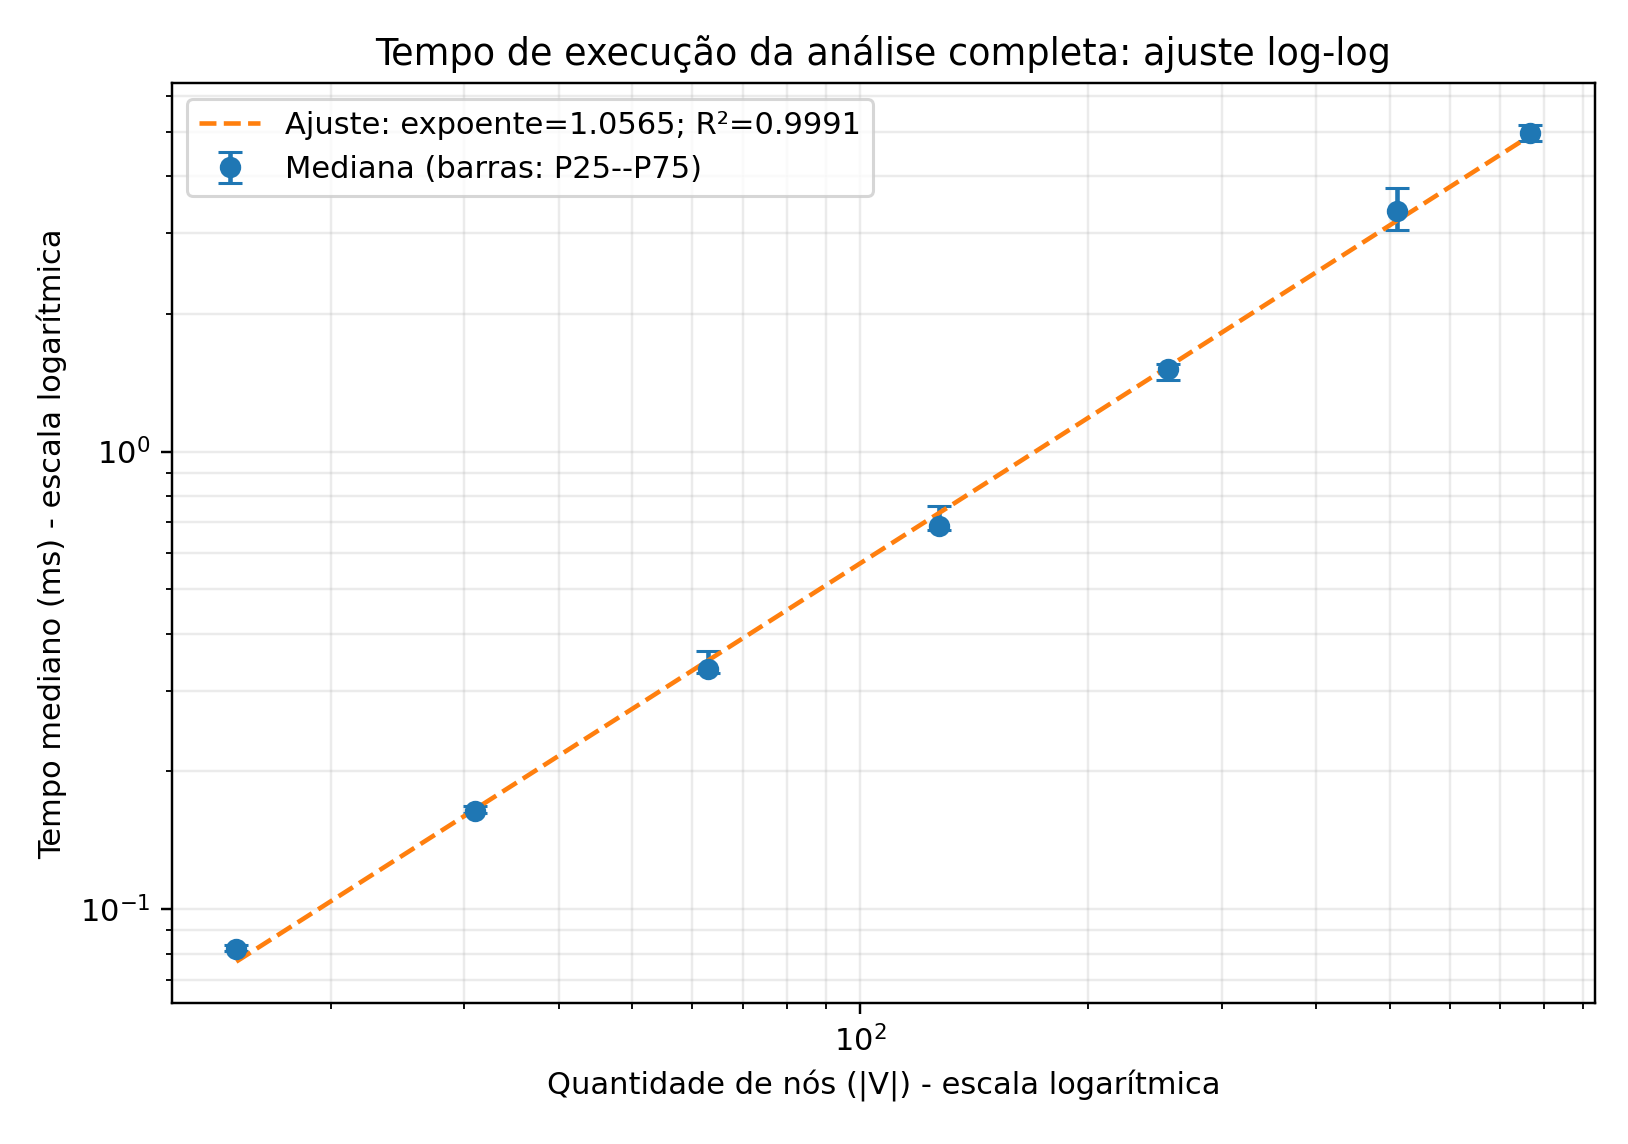
\includegraphics[width=0.88\textwidth]{benchmark_tempo.png}
\caption{Tempo mediano da análise completa em função da quantidade de nós, em escala log-log, com ajuste por mínimos quadrados ($\beta=1{,}0565$; $R^2=0{,}9991$).}
\label{fig:benchmark-tempo}
\fonte{Elaboração própria a partir de \texttt{benchmark\_complexidade.csv}.}
\end{figure}

\section{Limitações}
Embora o experimento abrangente avalie as quatro operações suportadas pelo motor, cada grafo experimental utiliza apenas uma operação repetida em todos os seus nós. Não foram avaliados grafos que misturam ADD, SUB, MUL e DIV em uma mesma expressão, nem grafos aleatórios ou aplicações extraídas de programas reais. Os tamanhos se limitam a 4, 8, 16 e 32 entradas; os valores nominais seguem uma sequência positiva específica e a perturbação relativa possui magnitude uniforme entre 50\% e 100\% do limite configurado.

A comparação entre cadeia e ramificada não isola a topologia nas operações SUB e DIV, pois a mudança de estrutura modifica a associação matemática. Para separar esses efeitos, um estudo posterior deverá construir grafos com a mesma função e os mesmos operandos, alterando apenas a organização do DAG.

Os casos determinísticos verificam reutilização de operandos e caminhos convergentes: no caso de $a^2$, a mesma entrada ocupa as duas posições de uma multiplicação; no caso de $(a+b)(ab)$, as entradas alimentam dois ramos que convergem na saída. Entretanto, os experimentos escalável e abrangente não avaliam, em larga escala, DAGs com compartilhamento de subexpressões intermediárias ou diferentes graus de saída (\textit{fan-out}). Assim, a validação da acumulação de sensibilidades em nós compartilhados permanece concentrada nos casos determinísticos e nos testes específicos. Uma avaliação futura com DAGs maiores e diferentes padrões de compartilhamento ampliaria a evidência experimental para essa propriedade.

Também não foram avaliados ciclos, desvios condicionais, operações transcendentes, entradas negativas ou denominadores próximos de zero, perturbações correlacionadas com distribuições alternativas, arredondamento de hardware ou modelos de ruído específicos de dispositivos.

A NRMSE e o MAPE possuem limitações quando as variações reais se aproximam de zero, conforme observado em algumas configurações. Embora os testes comparem as sensibilidades analíticas com diferenças finitas centrais, essa verificação valida o cálculo das derivadas e não constitui uma comparação experimental ampla entre métodos de aproximação. Não foi realizada uma linha de base sistemática com aritmética intervalar ou com outro estimador de propagação; essa comparação permanece como possibilidade de trabalho futuro. Os resultados, portanto, caracterizam o conjunto de funções, valores e perturbações efetivamente testado, e não devem ser generalizados automaticamente para todos os grafos aritméticos.

\chapter{CONSIDERAÇÕES FINAIS}

Este trabalho apresentou o desenvolvimento e a avaliação de um simulador para análise de propagação de erros em grafos direcionados acíclicos de fluxo de dados. O protótipo representa entradas e operações em nós, valida as dependências, avalia os valores, calcula derivadas locais e obtém sensibilidades globais por acumulação reversa. A implementação contempla adição, subtração, multiplicação e divisão e utiliza a regra da cadeia para acumular contribuições de nós compartilhados e caminhos convergentes.

A validação determinística aprovou os quatro casos de referência. Os dois arquivos de teste somaram 21 métodos aprovados na execução reproduzida. O Monte Carlo dos casos de referência gerou 12.000 amostras. O experimento escalável avaliou 16 configurações e 16.000 amostras, com correlações entre 0,999397 e 0,999999943 e RMSE empírico próximo da previsão teórica para a função de soma de produtos de pares.

O experimento abrangente avaliou 384 combinações e 384.000 amostras, sem amostras inválidas. As operações ADD e SUB apresentaram resíduos na ordem de $10^{-15}$, compatíveis com arredondamento de ponto flutuante; como cada função homogênea dessas operações é afim, a concordância da primeira ordem é esperada e serve como verificação de consistência, não como teste discriminante de aproximação em funções não lineares. Em MUL e DIV, os resultados mostraram maior dependência da intensidade, do tamanho do grafo e do padrão de sinais. O maior RMSE observado foi $6{,}1266\times10^{12}$, em uma cadeia de multiplicações com 32 entradas e perturbações positivas de 10\%. A menor correlação foi aproximadamente 0,95817, em uma árvore ramificada de multiplicações com 32 entradas e perturbações combinadas de 10\%.

Em conjunto, os experimentos sustentam que o motor calcula sensibilidades consistentes nos cenários testados e que a aproximação linear é adequada para funções afins e perturbações pequenas em diversos casos. Entretanto, a avaliação abrangente também demonstra que a primeira ordem pode ser insuficiente para funções não lineares sujeitas a perturbações relativas simultâneas, sobretudo em produtos de muitos operandos. A correlação, isoladamente, não substitui medidas de erro absoluto e normalizado, e métricas percentuais podem se tornar instáveis quando a variação real se aproxima de zero.

O benchmark complementar mediu cadeias de ADD entre 15 e 767 nós. O tempo mediano por nó variou de aproximadamente $5{,}45$\,\textmu s a $6{,}49$\,\textmu s, e o ajuste log-log apresentou expoente 1,06, em consonância com a análise $O(|V|+|E|)$ no intervalo observado. Essa medição complementa a demonstração assintótica, mas não prova experimentalmente a complexidade para todas as topologias e operações: foi realizada em uma única plataforma, em menos de duas ordens de grandeza e com cadeias de adição. Como continuidade, recomenda-se avaliar grafos com operações heterogêneas e funções extraídas de aplicações reais; comparar estruturas distintas mantendo a mesma expressão matemática, especialmente para SUB e DIV; ampliar as distribuições e os limites das perturbações; investigar aproximações de segunda ordem; estudar entradas negativas e denominadores próximos de zero; repetir o benchmark em outras plataformas e topologias; e substituir a ordenação recursiva por uma implementação iterativa para grafos muito profundos. A disponibilização conjunta dos códigos, testes, CSVs, referências bibliográficas por DOI e gráficos contribui para a reprodutibilidade da avaliação.

\postextual
\bibliographystyle{abntex2-alf}
\bibliography{referencias}

\begin{apendicesenv}
\chapter{DEDUÇÃO ALGÉBRICA DOS CASOS DETERMINÍSTICOS}

\section{Caso 1: perturbação em nó intermediário}
Considere $z=sc$, em que $s=a+b$ e $c=10$. A derivada em relação a $s$ é $\partial z/\partial s=c=10$. Para $\delta_s=0{,}5$, a estimativa linear é $10(0{,}5)=5$. Como a função é linear em $s$, a variação real também é 5 e o resíduo é zero.

\section{Caso 2: entrada repetida na multiplicação}
Para $z=a^2$, com $a=2$ e perturbação $\delta$, tem-se
\begin{equation}
\Delta z=(a+\delta)^2-a^2=2a\delta+\delta^2.
\end{equation}
A aproximação linear é $2a\delta$, de modo que $R=\delta^2$. Para $\delta=0{,}5$, o resíduo é $0{,}25$.

\section{Caso 3: caminhos convergentes}
Considere $z=(a+b)(ab)=a^2b+ab^2$. Ao perturbar apenas $a$ por $\delta$, mantendo $b$ fixo,
\begin{equation}
z(a+\delta,b)-z(a,b)=(2ab+b^2)\delta+b\delta^2.
\end{equation}
Para $a=2$ e $b=3$, a sensibilidade de $a$ é $2ab+b^2=21$ e o resíduo é $3\delta^2$. Com $\delta=0{,}5$, obtém-se $0{,}75$.

\section{Caso 4: perturbação no denominador}
Para $z=a/b$, com $a=12$, $b=3$ e perturbação $\delta$ no denominador,
\begin{equation}
\Delta z=\frac{12}{3+\delta}-4=-\frac{4\delta}{3+\delta}.
\end{equation}
A aproximação linear no ponto nominal é $-4\delta/3$. O resíduo é
\begin{equation}
R=-\frac{4\delta}{3+\delta}+\frac{4\delta}{3}=\frac{4\delta^2}{3(3+\delta)},
\end{equation}
para $\delta>-3$. Com $\delta=0{,}1$, o resíduo é $2/465$.

\chapter{INVENTÁRIO DOS ARQUIVOS DO PROJETO}
A Tabela~\ref{tab:inventario} relaciona os nomes normalizados utilizados para executar e reproduzir o projeto. As cópias que preservam os nomes da remessa original estão no subdiretório de originais; os nomes listados na tabela são os nomes canônicos utilizados nos comandos. Os artigos científicos externos são identificados pelas referências bibliográficas e pelos respectivos DOI, sem inclusão de cópias integrais no pacote.
\begin{longtable}{p{0.39\textwidth}p{0.53\textwidth}}
\caption{Inventário dos módulos, dados e materiais suplementares do projeto.}\label{tab:inventario}\\
\toprule
Arquivo no pacote & Descrição e utilização\\
\midrule
\endfirsthead
\toprule
Arquivo no pacote & Descrição e utilização\\
\midrule
\endhead
\arquivo{motor.py} & Classes \texttt{No} e \texttt{Motor}, avaliação, derivadas, sensibilidades e análise de perturbações.\\
\arquivo{casos.py} & Quatro grafos de referência e valores analíticos esperados.\\
\arquivo{main.py} & Execução e verificação dos quatro casos determinísticos.\\
\arquivo{monteCarlos.py} & Monte Carlo dos quatro casos, com 12.000 amostras.\\
\arquivo{monte\_carlo\_amostras.csv} & Dados individuais das 12.000 amostras dos casos de referência.\\
\arquivo{monte\_carlo\_resumo.csv} & Métricas agregadas por caso e intensidade no Monte Carlo de referência.\\
\arquivo{testes\_validacao.py} & Nove métodos de teste do conjunto principal.\\
\arquivo{testes\_validacao\_avancada.py} & Doze métodos de validação avançada.\\
\arquivo{experimento\_precisao.py} & Geração do experimento escalável com 16 configurações.\\
\arquivo{experimento\_amostras.csv} & Dados individuais das 16.000 amostras escaláveis.\\
\arquivo{experimento\_resumo.csv} & Métricas agregadas das 16 configurações escaláveis.\\
\arquivo{conferencia\_teorica.csv} & Conferência entre previsões teóricas e RMSE empírico do experimento escalável.\\
\arquivo{experimento\_abrangente.py} & Experimento com quatro operações, duas estruturas e 384 configurações.\\
\arquivo{abrangente\_amostras.csv} & 384.000 observações individuais do experimento abrangente.\\
\arquivo{abrangente\_resumo.csv} & 384 resumos das configurações experimentais.\\
\arquivo{abrangente\_intervalos.csv} & 384 intervalos aproximados de 95\% para o MAE.\\
\arquivo{abrangente\_amostra\_grafico.csv} & Subconjunto estratificado de 3.072 amostras usado na Figura 9.\\
\arquivo{validar\_residuos\_abrangente.py} & Verifica a convenção do resíduo por amostra e a média do viés nas 384 configurações.\\
\arquivo{CORRECAO\_RESIDUO.md} & Registro da correção do sinal e das verificações realizadas.\\
\arquivo{figuras/} & Figuras de precisão, comparação teórica, experimento abrangente e benchmark.\\
\arquivo{benchmark\_complexidade.py} & Benchmark complementar do tempo de execução de \texttt{Motor.analisar\_perturbacoes}.\\
\arquivo{benchmark\_complexidade.csv} & Tempos medidos para sete tamanhos de cadeia, com 30 repetições por tamanho.\\
\arquivo{gerar\_figuras.py} & Geração das figuras analíticas a partir dos CSVs, incluindo o ajuste log-log do benchmark.\\
\arquivo{requirements.txt} & Versões das bibliotecas externas utilizadas nos scripts de geração das figuras.\\
\arquivo{main.tex} & Fonte LaTeX da monografia.\\
\arquivo{referencias.bib} & Referências bibliográficas em formato BibTeX.\\
\arquivo{originais/} & Cópias preservadas dos arquivos de código, dados e gráficos com os nomes da remessa original.\\
\bottomrule
\end{longtable}

\chapter{REPRODUÇÃO E COMANDOS}
O material suplementar contém os módulos Python, os dados experimentais, os gráficos e os arquivos necessários à reprodução. Os artigos consultados são identificados na bibliografia por DOI; seus PDFs integrais não são redistribuídos no arquivo compactado. A execução de referência foi realizada com Python 3.13.5 em Linux x86\_64. As versões das bibliotecas utilizadas para gerar os gráficos foram Matplotlib 3.10.8, NumPy 2.3.5 e Pandas 2.2.3; os demais módulos do motor, dos testes, dos experimentos e do benchmark utilizam a biblioteca padrão do Python. As dependências de visualização podem ser instaladas com \texttt{python -m pip install -r requirements.txt}. O benchmark utiliza \texttt{time.perf\_counter\_ns} e não requer biblioteca externa.

Os códigos-fonte, dados experimentais e gráficos necessários à reprodução acompanham o material suplementar desta monografia. O material foi organizado para execução local, sem depender de um endereço público de repositório remoto.

Os comandos abaixo devem ser executados em uma pasta que contenha os arquivos normalizados:
\begin{verbatim}
python main.py
python -m unittest -v testes_validacao testes_validacao_avancada
python monteCarlos.py
python experimento_precisao.py
python experimento_abrangente.py
python benchmark_complexidade.py
python gerar_figuras.py
\end{verbatim}

Os CSVs do experimento abrangente integram os resultados analisados nesta monografia. Para reexecutar esse experimento, utilize o comando correspondente listado acima; ele executa as 384 combinações e gera os CSVs de amostras, resumo e intervalos, além dos gráficos agregados. Para produzir as figuras analíticas a partir dos CSVs existentes, sem repetir as simulações, execute o comando de geração de figuras também apresentado na lista. Os scripts podem sobrescrever resultados; preserve cópias antes de repetir os comandos.
\end{apendicesenv}

\end{document}
